%% rfam_prewarp_paper.tex
%% "Inverse Geometry Compensation and Turntable Exposure Averaging for
%%  Uniform Densification in Radio Frequency Additive Manufacturing"
%% Matthew McCoy, Georgia Institute of Technology
%% Compiled on Overleaf with pdflatex (elsarticle class)

\documentclass[5p,times]{elsarticle}

%% ---------------------------------------------------------------
%% Packages
%% ---------------------------------------------------------------
\usepackage{amsmath,amssymb,amsfonts}
\usepackage{graphicx}
\usepackage{booktabs}
\usepackage{multirow}
\usepackage{subcaption}
\usepackage{float}          % provides [H] specifier
\usepackage{placeins}      % provides \FloatBarrier
\usepackage{stfloats}      % allows figure* to use [b] and improves placement
\usepackage{siunitx}
\usepackage{xcolor}
\usepackage{microtype}
\usepackage[hidelinks,
            colorlinks=true,
            linkcolor=blue!60!black,
            citecolor=green!40!black,
            urlcolor=blue!60!black]{hyperref}
\usepackage[capitalise,noabbrev]{cleveref}
\usepackage{doi}    % makes DOI fields render as clickable https://doi.org/ links
\usepackage{caption}

%% ---------------------------------------------------------------
%% Graphics path  (flat figures/ folder — Overleaf compatible)
%% ---------------------------------------------------------------
\graphicspath{{figures/}}

%% ---------------------------------------------------------------
%% SI units configuration
%% ---------------------------------------------------------------
\sisetup{
  per-mode = symbol,
  detect-weight = true,
  detect-family = true
}

%% ---------------------------------------------------------------
%% Caption style
%% ---------------------------------------------------------------
\captionsetup{font=small, labelfont=bf, skip=4pt}

%% ---------------------------------------------------------------
%% Custom commands
%% ---------------------------------------------------------------
\newcommand{\Qrf}{Q_{\mathrm{rf}}}
\newcommand{\bndstd}{\sigma_{\mathrm{bnd}}}
\newcommand{\Leff}{L_{\mathrm{eff}}}
\newcommand{\rhorel}{\rho_{\mathrm{rel}}}
\newcommand{\Tpc}{T_{\mathrm{pc}}}
\newcommand{\phimelt}{\varphi}
\newcommand{\RMSE}{\mathrm{RMSE}}
\newcommand{\EPE}{\mathrm{EPE}}
\newcommand{\vect}[1]{\boldsymbol{#1}}
\newcommand{\nhat}{\hat{\vect{n}}}
\newcommand{\half}{\tfrac{1}{2}}

\begin{document}

\begin{frontmatter}

\title{Inverse Geometry Compensation and Turntable Exposure
Averaging for Uniform Densification in Radio Frequency Additive
Manufacturing}

\author[gatech]{Matthew McCoy}
\ead{matthew.mccoy@gatech.edu}
\address[gatech]{School of Mechanical Engineering, Georgia Institute of
Technology, Atlanta, Georgia 30332, USA}

\begin{abstract}
Radio Frequency Additive Manufacturing (RFAM) sinters graphite-doped
Nylon~12 powder at \SI{27.12}{\mega\hertz} by selective Joule
dissipation within the doped region.  Because the electro-quasi-static
(EQS) field is inherently non-uniform, the volumetric heating rate
$\Qrf = \half\sigma|\nabla V|^{2}$ varies by more than an order of
magnitude across the part cross-section: electric-field concentration
at geometric corners produces $\Qrf \approx 37\times$ the spatial
mean, normal-field enhancement at the faces perpendicular to the applied
electric field gives $\approx 11\times$, while the faces parallel to
the field couple only at $\approx 1.6\times$ the mean.  These gradients
drive spatial variation in melt fraction and post-sintering density that
causes both geometric distortion and structural non-uniformity in
finished parts.

This paper refreshes the RFAM compensation study around the current
HEATR physics stack: a complex-coefficient EQS solve, generator-power
scaled RF deposition, a DSC-calibrated apparent-heat-capacity melt
model for PA12, viscous-capillary densification, and explicit
energy-balance diagnostics.  The revised emphasis is therefore placed
on three result tiers that are currently supported by reusable
artifacts: (1) a 17-geometry single-exposure library screen,
(2) turntable benchmark runs on representative geometries, and
(3) one asymmetric orientation-optimizer showcase that addresses the
practical difficulty of physically rotating the loaded RFAM chamber.

The refreshed library screen preserves strong geometry-to-geometry
variation in melt fraction and density response while also exposing the
validation metrics now tracked by the solver.  Turntable rotation
remains an effective anisotropy-averaging benchmark, but it is now
discussed alongside the hardware constraint that the powder/part medium
must maintain electrode-facing contact to avoid introducing an
air-gap-capacitor-like impedance path during rotation.  For that
reason, the static orientation optimizer is positioned here as the more
practical deployment path.  Geometry prewarp and antennae energy
concentrators are retained only as reduced-status prototype sections:
legacy prewarp runs still show geometric error reduction on simple
shapes, but the prewarp workflow has not yet been fully refreshed on
the DSC-calibrated stack, and the current antennae study remains too
limited to support a strong improvement claim.
\end{abstract}

\begin{keyword}
Radio frequency additive manufacturing \sep inverse lithography \sep
geometry prewarp \sep edge placement error \sep turntable rotation \sep
Nylon~12 sintering \sep electro-quasi-static field \sep densification
uniformity
\end{keyword}

\end{frontmatter}

%% ---------------------------------------------------------------
\section{Introduction}
\label{sec:introduction}
%% ---------------------------------------------------------------

\subsection{The RFAM Process}

Radio Frequency Additive Manufacturing is a powder-bed sintering
process in which selective densification is achieved by incorporating
a conductive dopant---typically graphite---into a thermoplastic powder,
most commonly Nylon~12 (PA12).  The powder bed is placed between two
planar electrodes driven at the Industrial-Scientific-Medical (ISM)
frequency of \SI{27.12}{\mega\hertz}.  In the undoped regions the
powder is nearly lossless ($\sigma \approx 0$, $\varepsilon_r \approx
2$), so virtually no energy is absorbed.  In the doped regions the
effective conductivity rises to $\sigma \approx \SI{0.04}{\siemens\per\meter}$
and the relative permittivity to $\varepsilon_r \approx 20$, causing
selective Joule heating $\Qrf = \half\sigma|\vect{E}|^{2}$.  In the
current HEATR workflow, melting is modeled with a DSC-calibrated
apparent-heat-capacity representation of PA12 and densification is
advanced with a viscous-capillary law, so the transition from poured
powder density ($\rhorel \approx 0.55$) toward dense material is now
tied directly to the calibrated melt interval rather than to the older
nominal phase-window surrogate.

RFAM occupies a distinct niche among additive sintering processes.
Polymer powder-bed sintering was pioneered as selective laser sintering
(SLS) by Deckard~\cite{deckard1989method}, which relies on a scanned
laser beam to fuse each layer selectively~\cite{lupone2021process,bourell2014performance}.  Unlike SLS, RFAM energizes the \emph{entire}
doped region simultaneously using an ISM-band RF field~\cite{wroe1998rfmicrowave},
a fundamentally volumetric heating mechanism reviewed
in~\cite{Beaman2020AdditiveMR,gibson2015additive}.  This enables
rapid, potentially scalable throughput but introduces the fundamental
challenge addressed in this paper: the RF electromagnetic field is
spatially non-uniform, and this non-uniformity is encoded directly
into the sintered density distribution.

\subsection{The Two Coupled Problems}

Two distinct but related failure modes arise from RFAM's non-uniform
field:

\paragraph{Geometric distortion.}
Because densification implies volumetric shrinkage, and because the
degree of densification varies spatially, different parts of the
sintered boundary shrink by different amounts.  A nominally square
$20 \times \SI{20}{\milli\meter}$ target will emerge with corners
over-sintered and face midpoints under-sintered, producing a
systematically distorted outline.  Without compensation, the
root-mean-square boundary error is approximately \SI{0.68}{\milli\meter}
for the H-shape studied here---large enough to matter for any
fit-critical application.

\paragraph{Density non-uniformity.}
Even if geometric distortion is compensated by modifying the input
polygon, the underlying heating non-uniformity remains, producing
a part whose boundary density spans a factor of $\approx 1.46\times$
from the best-sintered corners to the worst-sintered parallel-field
face midpoints.  This density gradient is a structural defect that
cannot be corrected post hoc by shape changes alone.

\subsection{Prior Work}

The RFAM process was introduced and characterized physically by
Allison~\cite{allisonDissertation} and by Seepersad and
colleagues~\cite{allison2022volumetric,allison2022computational}, who
established the relationship between graphite doping concentration,
RF power, and sintering quality for Nylon~12.  More recently, Song
\textit{et al.}~\cite{Song2025RFAMUniformity} explored functional
grading of the doped region to improve heating uniformity, motivating
the geometry-level compensation approach developed here.  Computational
simulation of the coupled electromagnetic-thermal-densification
problem is developed in this work (see \cref{sec:methodology}) and shown to
reproduce the spatial pattern of COMSOL full-wave simulations at
significantly lower computational cost.

The concept of compensating for systematic process-induced distortions
by pre-modifying the design geometry is well established in optical
semiconductor lithography.  Optical proximity correction (OPC) and,
more recently, inverse lithography technology (ILT) iteratively modify
the photomask pattern so that diffraction, aberration, and resist
chemistry combine to print the desired target
feature~\cite{pang2021inverse,poonawala2007mask,chan2008initialization}.
The ILT field has seen rapid algorithmic progress over the past decade,
from EPE-gradient-descent methods~\cite{zhang2023fast} to
learning-to-optimize approaches~\cite{zhu2024l2o}.  To the authors'
knowledge, the ILT framework has not previously been applied to
RF-driven sintering.

Turntable-based exposure averaging in RF and microwave material
processing has been studied in the context of ceramic
sintering~\cite{RFceramic2023,ferdous2017rfheating} but has not been
combined quantitatively with geometric compensation for polymer
powder-bed RFAM.

\subsection{Contributions of This Paper}

This paper makes the following specific contributions:
\begin{enumerate}
\item A refreshed description of the current HEATR 2D EQS + thermal +
      DSC phase-change + viscous-capillary densification model for
      RFAM, including explicit validation/error diagnostics
      (\cref{sec:methodology}).
\item An EPE-based iterative prewarp algorithm adapted from ILT for
      arbitrary polygonal RFAM targets, with systematic $\Leff$
      calibration (\cref{sec:prewarp_algorithm}).
\item A systematic simulation study of 17 primitive shape geometries,
      characterizing the relationship between shape symmetry, boundary
      density non-uniformity, and melt fraction
      (\cref{sec:results_shapes}).
\item A refreshed 17-shape single-exposure screening dataset with
      explicit error columns for DSC consistency and nominal thermal /
      density mismatch (\cref{sec:results_shapes}).
\item A turntable benchmark discussion framed against practical RFAM
      chamber constraints, plus one orientation-optimizer showcase as a
      static alternative to mechanical rotation
      (\cref{sec:results_turntable,sec:lshape}).
\item Reduced-status prototype assessments of geometry prewarp and
      antennae energy concentrators, identifying the remaining gaps
      before those tools can be treated as mature results
      (\cref{sec:results_prewarp,sec:results_spikes}).
\end{enumerate}

%% ---------------------------------------------------------------
\FloatBarrier
\section{RFAM Physics and Field Non-Uniformity}
\label{sec:physics}
%% ---------------------------------------------------------------

\subsection{Joule Heating in an EQS Field}

At the RFAM operating frequency of \SI{27.12}{\mega\hertz}, the free-space
wavelength is $\lambda \approx \SI{11.1}{\meter}$, roughly 500 times
larger than the electrode spacing (\SI{22}{\milli\meter}).  The
displacement current term $\partial\vect{D}/\partial t$ is negligible
relative to the conduction current $\vect{J} = \sigma\vect{E}$ within
the doped region for $\sigma \gg \omega\varepsilon_0\varepsilon_r$
(which holds for $\sigma = \SI{0.04}{\siemens\per\meter}$ at
\SI{27.12}{\mega\hertz}).  The field therefore obeys the
electro-quasi-static (EQS) approximation:
\begin{equation}
  \nabla \cdot \left[\left(\sigma + j\omega\epsilon\right)\nabla V\right] = 0
  \label{eq:eqs_pde}
\end{equation}
with the instantaneous electric field $\vect{E} = -\nabla V$.  The
earlier conductivity-only shorthand used in older HEATR notes is
therefore best understood as a simplifying limit of the current
implementation, which retains the complex coefficient in the field
operator and then reports the deposited power through the real
time-averaged Joule-heating term.  The
time-averaged volumetric power deposition is:
\begin{equation}
  \Qrf = \half\,\sigma\,|\nabla V|^{2}
  \label{eq:qrf}
\end{equation}
where the factor of $\half$ accounts for time-averaging the sinusoidal
field $V(t) = V_0\cos(\omega t)$.  This coupled EQS-thermal formulation
is standard practice in RF and microwave materials processing
simulation~\cite{DielectricCeramicsPolymers,ferdous2017rfheating}; the
defining feature of RFAM relative to conventional microwave heating is
the high permittivity contrast between the graphite-doped part
($\varepsilon_r = 20$) and the surrounding powder ($\varepsilon_r = 2$),
which concentrates $\Qrf$ at geometric boundaries as described below.

\subsection{Physical Origin of Field Non-Uniformity}

The spatial variation of $\Qrf$ across a finite doped region can be
understood from three distinct physical mechanisms, each active at a
different part of the boundary.

\paragraph{Corners (37$\times$ mean).}
At a sharp convex corner between two material regions, the electric
field lines must turn through a larger angle than at a flat face.
For a corner of interior half-angle $\alpha$, the field is
amplified approximately as $r^{\pi/\alpha - 1}$ near the tip in a
lossless dielectric~\cite{Meixner1972singular}.  For a $90^\circ$
corner ($\alpha = \pi/2$), the exponent is $+1$, producing a $1/r$
field divergence as $r \to 0$ that concentrates energy strongly at
the tip.  This is the classical electrostatic tip-effect responsible
for lightning rods and field-emission tips, and it dominates the RFAM
heating pattern at all sharp vertices.

\paragraph{Perpendicular faces ($11\times$ mean).}
At an interface normal to the applied field ($z$-direction), the normal
component of $\vect{D} = \varepsilon_r\varepsilon_0\vect{E}$ is
continuous across the boundary.  Therefore:
\begin{equation}
  \varepsilon_{r,\mathrm{doped}}\,E_{n,\mathrm{in}} =
  \varepsilon_{r,\mathrm{powder}}\,E_{n,\mathrm{out}}
  \label{eq:normal_D_continuity}
\end{equation}
giving $E_{n,\mathrm{in}} = (\varepsilon_{r,\mathrm{powder}} /
\varepsilon_{r,\mathrm{doped}})\,E_{n,\mathrm{out}}$.  For
$\varepsilon_{r,\mathrm{doped}} = 20$ and $\varepsilon_{r,\mathrm{powder}} = 2$,
the interior normal field is \emph{reduced} by a factor of 10 compared
to the exterior, but the $\Qrf \propto |E|^{2}$ evaluated inside the
doped region still shows a substantial enhancement over the center
because the exterior field itself is enhanced by the overall
dielectric contrast.  Numerically, the net effect at the top and
bottom face midpoints is $\approx 11\times$ the spatial mean of
$\Qrf$ across the part.

\paragraph{Parallel faces (1.6$\times$ mean).}
At an interface parallel to the applied field, the tangential component
of $\vect{E}$ is continuous:
\begin{equation}
  E_{t,\mathrm{in}} = E_{t,\mathrm{out}}
  \label{eq:tangential_E_continuity}
\end{equation}
There is no field concentration mechanism; the interior field at the
face midpoint is essentially equal to the far-field value of
$\approx 860/60 = \SI{14.3}{\volt\per\milli\meter}$.  The mild
enhancement of $\approx 1.6\times$ arises from the global redistribution
of field lines around the high-permittivity doped region
(depolarization effect), not from any boundary-normal concentration.

\subsection{Consequences for Sintering}

The $37\times$ ratio between corner and center $\Qrf$ means that
corners reach the melt threshold ($\sim\SI{180}{\celsius}$) far earlier
than the face midpoints and substantially earlier than the part
interior.  At the 6-minute canonical exposure time, corners have
$\rhorel \approx 0.80$ while the parallel-field face midpoints barely
reach $\rhorel \approx 0.55$ (initial poured density).  This spatial
gradient in sintering extent is the root cause of both dimensional
distortion and structural non-uniformity.

%% ---------------------------------------------------------------
\FloatBarrier
\section{Methodology}
\label{sec:methodology}
%% ---------------------------------------------------------------

\subsection{Electro-Quasi-Static Forward Model}
\label{sec:eqs_model}

\subsubsection{Governing Equation and Discretization}

\Cref{eq:eqs_pde} is solved on a 2D Cartesian grid representing the
XZ cross-section (horizontal = $x$, vertical = $z$, electrodes on the
$z$-axis).  The domain is $60 \times \SI{60}{\milli\meter}$ with
$120 \times 120$ uniform cells ($\Delta x = \Delta z \approx
\SI{0.504}{\milli\meter}$).  The part occupies a $20 \times
\SI{20}{\milli\meter}$ square at the center; the surrounding
\SI{20}{\milli\meter}-wide annular region is undoped powder.

The discretization uses a standard finite-difference stencil for
\cref{eq:eqs_pde} on the Cartesian grid.  In the current HEATR code
path, the complex material coefficient $(\sigma + j\omega\epsilon)$ is
assembled cellwise so that both conductive and displacement
contributions appear in the EQS operator.  The resulting sparse linear
system is assembled in CSR format and solved via
\texttt{scipy.sparse.linalg.spsolve} (SuperLU backend).

\subsubsection{Boundary Conditions}

The electrode boundary conditions are:
\begin{align}
  V &= 0 \quad \text{at } z = +\SI{30}{\milli\meter} \quad
       \text{(top electrode)} \label{eq:bc_top}\\
  V &= V_0 = \SI{860}{\volt} \quad \text{at } z = -\SI{30}{\milli\meter}
       \quad \text{(bottom electrode)} \label{eq:bc_bot}
\end{align}
matching the COMSOL reference model (Tuned\_Sigma.mph).  The lateral
boundaries ($x = \pm\SI{30}{\milli\meter}$) use Neumann conditions
$\partial V/\partial x = 0$ (zero normal current, representing
insulating chamber walls).

\subsubsection{Power Normalization}

The generator delivers $P_{\mathrm{gen}} = \SI{500}{\watt}$ to the
system.  Due to impedance mismatch and coupling losses between the
generator and the powder-bed load, the effective power absorbed by the
doped region is enforced through:
\begin{equation}
  P_{\mathrm{eff}} = \eta\,P_{\mathrm{gen}}\,/\,d_{\mathrm{eff}}
  \label{eq:power_eff}
\end{equation}
where $\eta = 0.020$ (2\% coupling efficiency, calibrated to match
COMSOL steady-state temperatures) and $d_{\mathrm{eff}} =
\SI{0.020}{\meter}$ is the effective part depth in the out-of-plane
direction.  After each EQS solve, the $\Qrf$ map is scaled such that
$\int_\Omega \Qrf\,\mathrm{d}A = P_{\mathrm{eff}}$.  This keeps the
RF source consistent with the selected generator model regardless of
the instantaneous part geometry and field intensity distribution.

The EQS solve is repeated every 20 thermal time steps (\SI{10}{\second})
to capture the effect of temperature-dependent material properties.
In practice, the present refreshed result set uses constant electrical
properties for the doped region, so the EQS solution changes primarily
with geometry and turntable/orientation remapping rather than through a
strong temperature-dependent conductivity feedback.

\subsection{Thermal Model}
\label{sec:thermal_model}

The transient heat equation with apparent-heat-capacity treatment of
phase change is:
\begin{equation}
  \rho_{\mathrm{mat}}\,c_p^{\mathrm{eff}}\,\frac{\partial T}{\partial t}
  = \nabla\cdot(k\,\nabla T) + \Qrf - h_c\,(T - T_\infty)\,\delta_{\mathrm{top}}
  \label{eq:heat_eqn}
\end{equation}
where $\delta_{\mathrm{top}}$ is 1 on the top boundary and 0
elsewhere.  The apparent specific heat absorbs the latent heat of
fusion $\mathcal{L}$ over a smoothed phase-change interval $\Delta T$:
\begin{equation}
  c_p^{\mathrm{eff}}(T) = c_p + \mathcal{L}\,
  \frac{1}{\Delta T}\,H'\!\left(\frac{T - \Tpc}{\Delta T}\right)
  \label{eq:apparent_cp}
\end{equation}
where $H'$ is a smoothed transition kernel.  In the current
DSC-calibrated PA12 model family, the melt interval is represented by
$T_{\mathrm{onset}} = \SI{171.0}{\celsius}$,
$T_{\mathrm{peak}} = \SI{180.8}{\celsius}$,
$T_{\mathrm{end}} = \SI{186.0}{\celsius}$, and
$\mathcal{L} = \SI{101700}{\joule\per\kilogram}$ rather than by the
older nominal $\SI{180}{\celsius}\pm\SI{5}{\celsius}$ surrogate.

Material properties are blended between the solid and liquid phases
based on the local melt fraction $\phimelt \in [0, 1]$, where
$\phimelt = H((T - \Tpc)/\Delta T)$:
\begin{align}
  k(T) &= (1-\phimelt)\,k_s + \phimelt\,k_l \\
  \rho_{\mathrm{mat}}(T) &= (1-\phimelt)\,\rho_s + \phimelt\,\rho_l
\end{align}
Table~\ref{tab:material_props} summarizes all material constants.
Convection is applied only on the top face with $h_c =
\SI{5}{\watt\per\meter\squared\per\kelvin}$ and
$T_\infty = \SI{23}{\celsius}$ in the refreshed default configuration;
all other boundaries are adiabatic.  The current solver advances the
thermal field with an outer step of $\Delta t = \SI{0.5}{\second}$,
stability-controlled substepping, and a cumulative energy-balance
diagnostic reported at the end of each run.

\begin{table}[tb]
\centering
\caption{Material properties for Nylon~12 and graphite-doped powder
         used in the RFAM forward model.
         Solid-phase and liquid-phase thermal properties from
         \cite{allisonDissertation,allison2022computational};
         powder bulk properties from \cite{verbelen2016characterization};
         phase-change parameters from \cite{zarringhalam2006effects,zhao2018crystallization}.}
\label{tab:material_props}
\begin{tabular}{llSl}
\toprule
Property & Symbol & {Value} & {Unit} \\
\midrule
\multicolumn{4}{l}{\textit{Nylon 12 powder (undoped)}} \\
Thermal conductivity & $k_p$ & 0.197 & \si{\watt\per\meter\per\kelvin} \\
Density & $\rho_p$ & 490 & \si{\kilogram\per\meter\cubed} \\
Specific heat & $c_{p,p}$ & 1072 & \si{\joule\per\kilogram\per\kelvin} \\
\midrule
\multicolumn{4}{l}{\textit{Nylon 12 doped solid}} \\
Thermal conductivity & $k_s$ & 0.10 & \si{\watt\per\meter\per\kelvin} \\
Density & $\rho_s$ & 460 & \si{\kilogram\per\meter\cubed} \\
Specific heat & $c_{p,s}$ & 2500 & \si{\joule\per\kilogram\per\kelvin} \\
Electrical conductivity & $\sigma$ & 0.04 & \si{\siemens\per\meter} \\
Relative permittivity & $\varepsilon_r$ & 20 & {---} \\
\midrule
\multicolumn{4}{l}{\textit{Nylon 12 doped liquid}} \\
Thermal conductivity & $k_l$ & 0.26 & \si{\watt\per\meter\per\kelvin} \\
Density & $\rho_l$ & 1010 & \si{\kilogram\per\meter\cubed} \\
Specific heat & $c_{p,l}$ & 3279 & \si{\joule\per\kilogram\per\kelvin} \\
\midrule
\multicolumn{4}{l}{\textit{DSC-calibrated phase change}} \\
Melt onset & $T_{\mathrm{onset}}$ & 171.0 & \si{\celsius} \\
Melt peak & $T_{\mathrm{peak}}$ & 180.8 & \si{\celsius} \\
Melt end & $T_{\mathrm{end}}$ & 186.0 & \si{\celsius} \\
Latent heat & $\mathcal{L}$ & 101700 & \si{\joule\per\kilogram} \\
\midrule
\multicolumn{4}{l}{\textit{Generator / coupling}} \\
Generator power & $P_{\mathrm{gen}}$ & 500 & \si{\watt} \\
Coupling efficiency & $\eta$ & 0.020 & {---} \\
Effective depth & $d_{\mathrm{eff}}$ & 0.020 & \si{\meter} \\
\bottomrule
\end{tabular}
\end{table}

\subsection{Densification Model}
\label{sec:densification_model}

The relative density field $\rhorel(x,z,t)$ in the current default
model family is evolved with a viscous-capillary PA12 densification law
rather than the older dual-Arrhenius surrogate.  The liquid-regime
mobility is controlled by a temperature-dependent viscosity, modeled in
the refreshed default stack with an Arrhenius form:
\begin{equation}
  \eta(T) = \eta_{\mathrm{ref}}
  \exp\!\left[\frac{E_a}{R}\left(\frac{1}{T} -
  \frac{1}{T_{\mathrm{ref}}}\right)\right]
  \label{eq:viscosity_arrhenius}
\end{equation}
using $\eta_{\mathrm{ref}} = \SI{8000}{\pascal\second}$,
$T_{\mathrm{ref}} = \SI{458.15}{\kelvin}$,
$E_a = \SI{60000}{\joule\per\mol}$, surface tension
$\gamma = \SI{0.03}{\newton\per\meter}$, particle radius
$r_p = \SI{35}{\micro\meter}$, melt-fraction threshold 0.02, and
geometry factor 0.05.  This is the model family exposed in the current
GUI as the DSC-calibrated PA12 default.

The practical implication for this paper is that the refreshed
single-exposure, turntable, and orientation-optimizer results should be
interpreted through this viscous-capillary description rather than
through the older two-branch kinetics.  The initial density remains
$\rhorel(t=0) = 0.55$ uniformly throughout the doped region, matching
the bulk poured density of graphite-doped PA12 powder~\cite{verbelen2016characterization}.

\subsection{Validation and Error Metrics}
\label{sec:validation_metrics}

The updated paper also reports the numerical diagnostics now tracked by
HEATR.  In addition to geometric RMSE or boundary-density-uniformity
metrics, the refreshed tables surface an energy-balance residual and,
for the reusable 17-shape screening dataset, DSC plausibility and
nominal thermal / density mismatch columns.  These error measures are
included to make clear which updated results are mature and which remain
prototype-quality.

\subsection{EPE-Based Geometry Prewarp Algorithm}
\label{sec:prewarp_algorithm}

\subsubsection{Analogy to Inverse Lithography Technology}

In optical semiconductor lithography, the target pattern on the wafer
is related to the mask pattern by a forward operator $\mathcal{F}$
representing diffraction, lens aberrations, and resist chemistry.  ILT
seeks the mask $M^*$ such that $\mathcal{F}(M^*) \approx T$, where
$T$ is the target wafer pattern.  The standard iterative solution
uses gradient descent on the edge placement error:
$\EPE[i] = (\vect{T}[i] - \hat{\vect{B}}[i]) \cdot \nhat_{\mathrm{out}}[i]$,
where $\hat{\vect{B}}$ is the predicted printed boundary and
$\vect{T}[i]$ is the nearest target boundary point.

For RFAM, the analogous forward operator maps the input polygon $P$
through (a) EQS+thermal sintering simulation, (b) local shrinkage, and
(c) final boundary prediction to yield an estimated sintered boundary
$\hat{\vect{B}}$.  The prewarp algorithm iteratively adjusts $P$ to
minimize $\EPE$ in the same spirit as optical ILT.

\subsubsection{Algorithm}

Let $T$ be the target polygon (desired sintered shape) and $P_k$ be
the prewarp polygon at iteration $k$, both represented as ordered
lists of $N = 512$ equally-spaced vertices.  The algorithm proceeds
as follows:

\begin{enumerate}
\item \textbf{Initialize:} $P_0 = T$.
\item \textbf{Forward simulation:} Run the EQS+thermal+densification
      model on polygon $P_k$ for $t = \SI{360}{\second}$.
\item \textbf{Boundary density sampling:} For each vertex $i$, compute
      the outward normal $\nhat_i$.  Sample $\rhorel$ at a point
      inset $\approx 1.5$ grid cells inward along $\nhat_i$:
      $\rhorel^{\mathrm{bnd}}[i]$.
\item \textbf{Shrinkage prediction:} Estimate the local linear
      shrinkage ratio from the measured boundary density, assuming
      isotropic densification from initial density $\rhorel^{(0)}$:
      \begin{equation}
        s[i] = 1 - \sqrt{\rhorel^{(0)}\,/\,\rhorel^{\mathrm{bnd}}[i]}
        \label{eq:shrinkage_ratio}
      \end{equation}
\item \textbf{Predicted boundary:} Project each vertex outward by the
      shrinkage distance:
      \begin{equation}
        \hat{\vect{B}}[i] = P_k[i] - s[i]\,\Leff\,\nhat_i
        \label{eq:predicted_boundary}
      \end{equation}
      where $\Leff$ is the effective shrinkage length scale
      (calibrated parameter, \cref{sec:leff_calibration}).
\item \textbf{Edge placement error:}
      \begin{equation}
        \EPE[i] = (T[i] - \hat{\vect{B}}[i]) \cdot \nhat_i
        \label{eq:epe}
      \end{equation}
\item \textbf{Polygon update:}
      \begin{equation}
        P_{k+1}[i] = P_k[i] + \alpha\,\EPE[i]\,\nhat_i
        \label{eq:polygon_update}
      \end{equation}
      where $\alpha = 1.0$ is the step size (unit EPE-to-correction
      ratio, justified by the approximately linear relationship between
      input polygon boundary position and sintered boundary position
      for small perturbations).
\item \textbf{Laplacian smoothing:}
      \begin{equation}
        P_{k+1}[i] \leftarrow P_{k+1}[i] +
        \lambda_s\,\bigl(P_{k+1}[i-1] - 2P_{k+1}[i] + P_{k+1}[i+1]\bigr)
        \label{eq:laplacian_smooth}
      \end{equation}
      with $\lambda_s = 0.15$, applied 3 times to suppress
      high-frequency oscillations that arise at vertices where
      $\EPE$ is noisy.
\item \textbf{Resample:} Re-parameterize $P_{k+1}$ to $N = 512$
      equally-spaced vertices by arc-length.
\item \textbf{Convergence check:} Stop if
      $\mathrm{RMS}(\EPE) < \varepsilon_{\EPE}$, with
      $\varepsilon_{\EPE} = \SI{0.25}{\milli\meter}$ for square/circle
      and \SI{0.30}{\milli\meter} for the H-shape.
\end{enumerate}

\subsubsection{$\Leff$ Calibration}
\label{sec:leff_calibration}

The effective shrinkage length $\Leff$ is the only free parameter of
the prewarp algorithm.  Physically, it represents the characteristic
distance over which the boundary density $\rhorel^{\mathrm{bnd}}$
measured at the vertex inset point translates into a linear shrinkage
at the sintered boundary.  It depends on the exposure time, material
properties, and the local $\Qrf$ gradient near the boundary, and
therefore differs between shapes.

Calibration is performed by running the full prewarp algorithm to
convergence for each candidate $\Leff \in \{3, 5, 7, 10, 13, 16\}
\si{\milli\meter}$ and selecting the value that achieves the lowest
post-convergence geometric RMSE:
\begin{equation}
  \RMSE = \sqrt{\frac{1}{N}\sum_{i=1}^{N}\EPE[i]^{2}}
  \label{eq:rmse}
\end{equation}

\subsection{Boundary Density Uniformity Metrics}
\label{sec:uniformity_metrics}

Two complementary scalar metrics quantify the spatial uniformity of
sintering across the part boundary.

\paragraph{Boundary standard deviation.}
The one-cell-thick boundary mask $\mathcal{B}$ is defined as the
set-difference between the part mask and its binary erosion:
\begin{equation}
  \mathcal{B} = \{(i,j) : M_{ij} = 1\} \setminus
                \mathrm{erode}(\{(i,j) : M_{ij} = 1\})
  \label{eq:boundary_mask}
\end{equation}
The boundary standard deviation is then:
\begin{equation}
  \bndstd = \mathrm{std}\bigl(\{\rhorel[i,j] : (i,j)\in\mathcal{B}\}\bigr)
  \label{eq:bnd_std}
\end{equation}
Lower $\bndstd$ indicates more uniform surface sintering.

\paragraph{Min/max ratio.}
\begin{equation}
  r_{\mathrm{bnd}} = \frac{\min_{(i,j)\in\mathcal{B}}\rhorel[i,j]}
                         {\max_{(i,j)\in\mathcal{B}}\rhorel[i,j]}
  \in [0, 1]
  \label{eq:minmax_ratio}
\end{equation}
$r_{\mathrm{bnd}} \to 1$ implies perfectly uniform boundary density.
This metric is complementary to $\bndstd$ in that it captures the
worst-case nonuniformity rather than the distribution spread.

\subsection{Antennae Energy Concentrator Geometry}
\label{sec:spike_method}

Sub-resolution assist features (SRAFs) in optical lithography are mask
elements that are too small to print but that improve the aerial image
intensity distribution for nearby features they are designed to
assist~\cite{pang2021inverse}.  The RFAM analog is a narrow convex
protrusion at a region of under-heating (a parallel-to-$\vect{E}$ face
midpoint) that concentrates $\vect{E}$ locally through the same tip
effect responsible for corner overheating, with the intent of
increasing $\Qrf$ at the face midpoint without contributing significant
sintered material.

Each antenna is defined as a radial perturbation to the polygon at a
specified angular location $\theta_0$:
\begin{equation}
  \delta r(\theta) = h\,\exp\!\!\left(-\frac{(\theta-\theta_0)^2}{2\sigma_s^2}\right)
  \label{eq:spike_profile}
\end{equation}
where $h$ is the antenna height (parameter to optimize),
$\sigma_s = w_{\mathrm{base}} / (2\sqrt{2\ln 2})$ is the Gaussian
width parameter, and $w_{\mathrm{base}}$ is the full-width-at-half-maximum
angular extent.  A narrow angular width $w_{\mathrm{base}} = 10^\circ$
is used to maximize field concentration effect per unit area added to
the polygon.  Antennae are placed at $\theta_0 = 0^\circ$ and
$180^\circ$ (the two parallel-to-$\vect{E}$ face midpoints of the
square).

\subsection{Turntable Rotation Model}
\label{sec:turntable_method}

The physical scenario is a motorized turntable that rotates the entire
part assembly---the doped-region polygon rasterized on the powder
bed---at discrete angles within the fixed RF field (electrodes remain
stationary).  Rotation is discrete (not continuous) because a
continuous rotation would sweep each boundary element through all
field orientations simultaneously, which is equivalent to perfect
averaging and is the upper limit of what rotation can achieve.

At each rotation event at time $t_k$, the cumulative rotation angle
is incremented by $\Delta\theta = 90^\circ$, and the spatial fields
$(T, \rhorel, \phimelt)$ are remapped from the old to the new grid:
\begin{equation}
  f^{\mathrm{new}}(x, z) = f^{\mathrm{old}}(R_{-\Delta\theta}(x,z))
  \label{eq:rotation_remap}
\end{equation}
where $R_{-\Delta\theta}$ is the inverse rotation operator.  The
remapping uses bilinear interpolation via
\texttt{scipy.ndimage.map\_coordinates}, which preserves the spatial
structure of hot-spots and density gradients with sub-grid accuracy.

The rotation schedule is time-based rather than melt-fraction-based
(the latter would require real-time density sensing):
\begin{equation}
  t_k = \frac{k}{N_r + 1}\,t_{\mathrm{total}},
  \quad k = 1, 2, \ldots, N_r
  \label{eq:rotation_schedule}
\end{equation}
For $N_r = 4$ rotations over $t_{\mathrm{total}} = \SI{360}{\second}$:
rotations occur at $t = 72, 144, 216, 288\,\si{\second}$, each adding
$90^\circ$ for a total of $360^\circ$ over the full exposure.  This
schedule is uniformly spaced so that each of the four $90^\circ$
orientations occupies an equal $\SI{72}{\second}$ interval.

%% ---------------------------------------------------------------
\FloatBarrier
\section{Canonical Baseline Results}
\label{sec:results_baseline}
%% ---------------------------------------------------------------

\subsection{EQS Field Distribution: 20 mm Square at 6 Minutes}

\Cref{fig:canonical_fields} presents the canonical simulation result
for a $20 \times \SI{20}{\milli\meter}$ square at $t = \SI{360}{\second}$.
The electric potential $|V|$ shows the expected near-linear gradient
between electrodes, slightly distorted by the high-permittivity doped
region.  The $\Qrf$ map reveals the characteristic non-uniformity
driven by the three mechanisms described in \cref{sec:physics}:
corners at $\approx 37\times$ the spatial mean, perpendicular faces at
$\approx 11\times$, and parallel faces at $\approx 1.6\times$.  The
numerical values of $\Qrf$ at representative locations are listed in
\cref{tab:qrf_values}.

\begin{figure}[H]
  \centering
  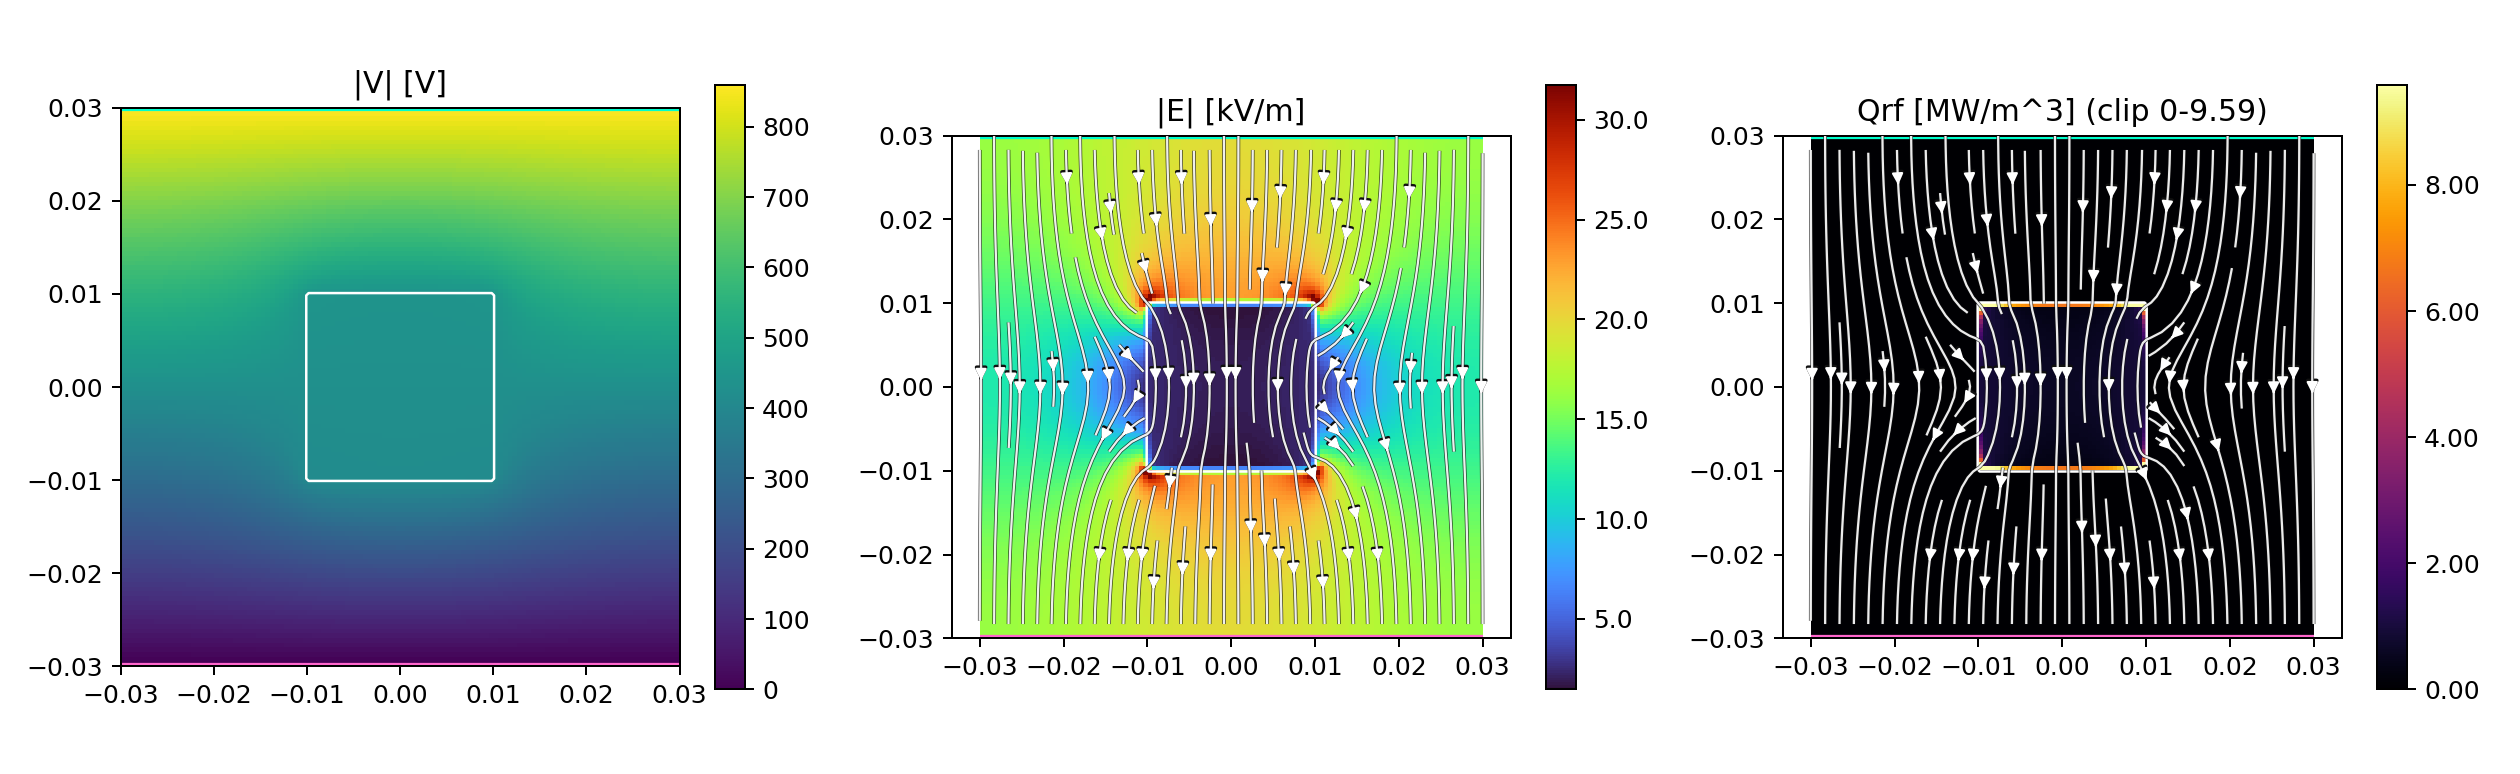
\includegraphics[width=\columnwidth]{fig_electric_fields.png}
  \caption{Canonical 6-minute run: electric potential $|V|$, electric field
           magnitude $|\vect{E}|$, and volumetric RF heating rate $\Qrf$ for
           a $20\times\SI{20}{\milli\meter}$ square.  The $\approx 37\times$
           corner-to-center ratio in $\Qrf$ is evident.  Chamber:
           $60\times\SI{60}{\milli\meter}$; generator: \SI{500}{\watt}, 2\%
           coupling efficiency.}
  \label{fig:canonical_fields}
\end{figure}

\begin{table}[tb]
\centering
\caption{Volumetric RF heating rate $\Qrf$ at representative boundary
         locations for the 20~mm square at $t = \SI{360}{\second}$.
         Ratios are relative to the spatial mean over the doped region.}
\label{tab:qrf_values}
\begin{tabular}{lSS[table-format=2.0]}
\toprule
Location & {$\Qrf$ (\si{\watt\per\meter\cubed})} & {Ratio to mean} \\
\midrule
Corner & 2.26e9 & 37 \\
Top/bottom face midpoint & 3.34e8 & 11 \\
Left/right face midpoint & 4.77e7 & 1.6 \\
Part center & 3.13e7 & 1.0 \\
\bottomrule
\end{tabular}
\end{table}

\begin{figure*}[!t]
  \centering
  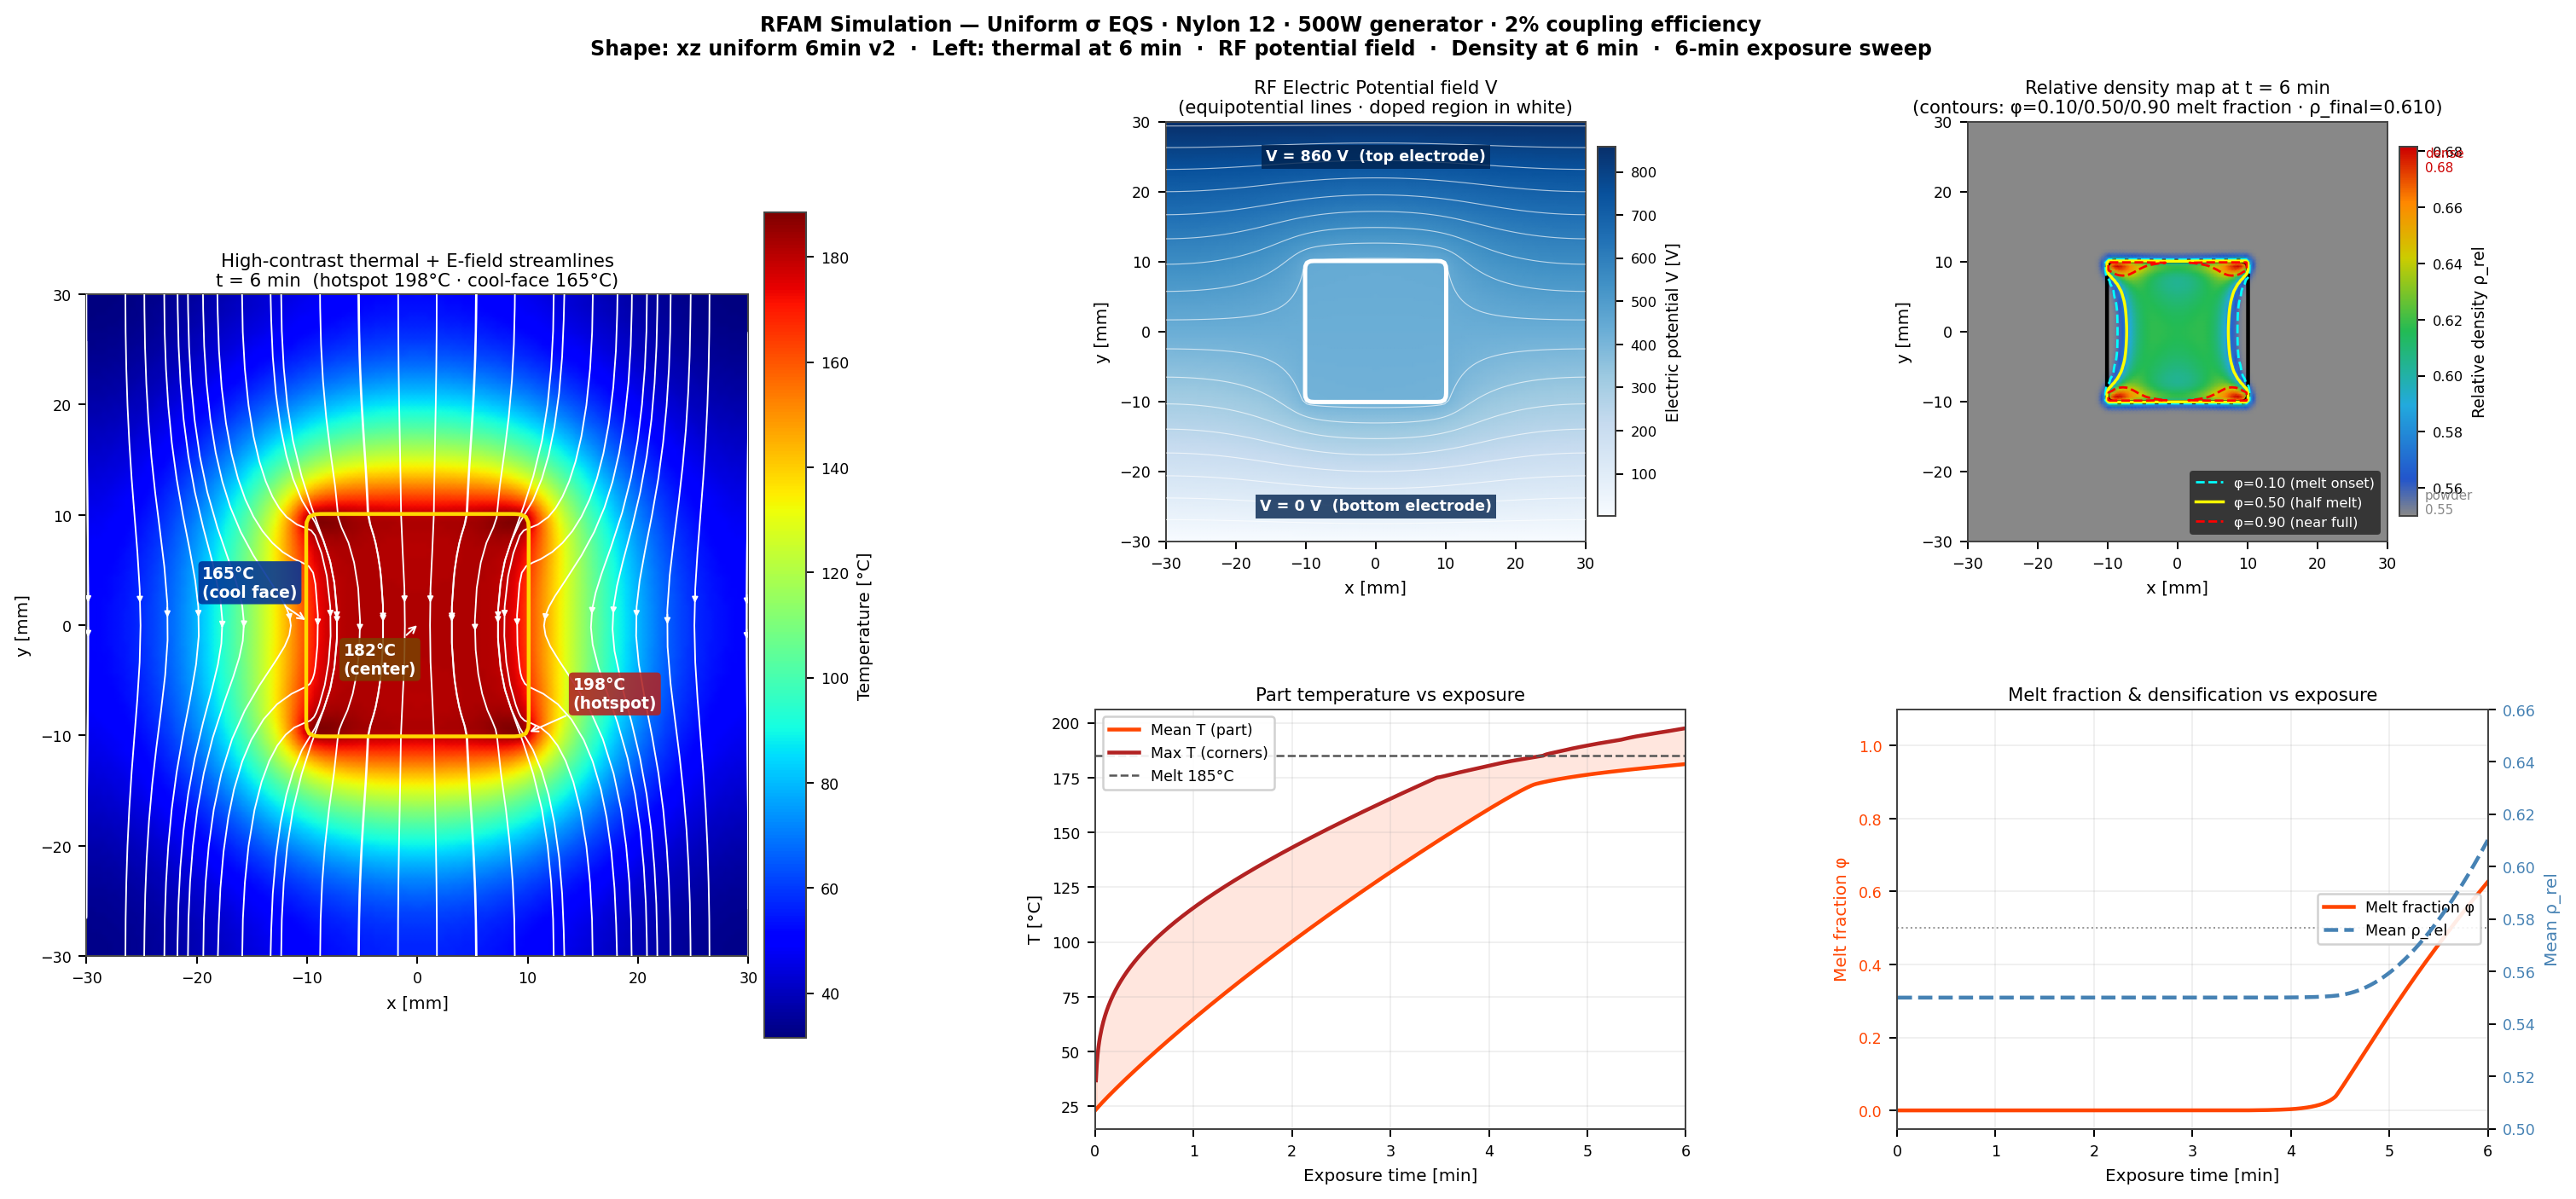
\includegraphics[width=\textwidth]{fig_canonical_v5.png}
  \caption{Canonical five-panel summary for the $20\times\SI{20}{\milli\meter}$
           square at $t = \SI{360}{\second}$ (6 min).
           (A)~Temperature field (jet colormap) with E-field streamlines;
           (B)~RF electric potential $|V|$ with equipotential lines and
           electrode labels (top: $V = 0$, bottom: $V = 860$ V);
           (C)~relative density $\rhorel$ with melt-front contours at
           $\phimelt = 0.10$ (dashed cyan), $0.50$ (solid yellow), $0.90$
           (dashed red);
           (D)~mean part temperature vs.\ exposure time;
           (E)~mean melt fraction $\bar{\phimelt}$ and mean relative density
           $\bar{\rhorel}$ vs.\ time.
           The spatial non-uniformity in $\rhorel$
           ($\mathrm{UI}_\mathrm{rms} = 0.235$) driven by the corner/face
           $\Qrf$ gradient is clearly visible.}
  \label{fig:canonical_full}
\end{figure*}

\subsection{Thermal and Density Results}

\Cref{fig:canonical_full} presents the five-panel canonical result.
At $t = \SI{360}{\second}$:
\begin{itemize}
  \item Mean temperature: $\bar{T} = \SI{181.2}{\celsius}$;
        maximum: $T_{\max} = \SI{197.6}{\celsius}$
  \item Mean melt fraction: $\bar{\phimelt} = 0.626$;
        fraction of cells at $T \geq T_{\mathrm{pc}}$: 82.5\%
  \item Mean relative density: $\bar{\rhorel} = 0.610$
  \item Boundary density metrics: $\bndstd = 0.072$,
        $r_{\mathrm{bnd}} = 0.699$
\end{itemize}
The temperature field shows local hot-spots at corners reaching
$\SI{197.6}{\celsius}$ while parallel-face midpoints approach the
melt threshold from below.  The density field shows the same pattern
amplified by the non-linear densification kinetics: corners at
$\rhorel \approx 0.80$ vs. parallel-face midpoints at
$\rhorel \approx 0.55$.

\subsection{Time-Exposure Sweep: 6--10 Minutes}

\Cref{tab:time_sweep} presents the systematic time-exposure sweep,
demonstrating how all state variables evolve with exposure time for
the canonical square geometry.  The melt fraction $\bar{\phimelt}$
increases rapidly from 6 to 8 minutes (0.626 to 0.964) and saturates
near 1.0 by 9 minutes, while the relative density continues to increase
more slowly (0.610 to 0.932 over the full 4-minute window).  The
boundary density standard deviation $\bndstd$ monotonically increases
with exposure time: as the already-hot corners advance into the
liquid-state sintering regime and the parallel faces merely enter
solid-state sintering, the density gap between these regions widens.

\begin{table*}[tb]
\centering
\caption{Time-exposure sweep for the canonical $20\times\SI{20}{\milli\meter}$
         square at \SI{500}{\watt}, 2\% coupling efficiency.  $\bar{\phimelt}$
         is the spatial mean melt fraction over the part domain;
         $\bar{\rhorel}$ is the spatial mean relative density.}
\label{tab:time_sweep}
\begin{tabular}{cSSSSS}
\toprule
$t$ (min) & {$\bar{T}$ (\si{\celsius})} & {$T_{\max}$ (\si{\celsius})}
           & {$\bar{\phimelt}$} & {$\bar{\rhorel}$} & {$\bndstd$} \\
\midrule
6  & 181.2 & 197.6 & 0.626 & 0.610 & 0.0724 \\
7  & 185.9 & 205.9 & 0.894 & 0.692 & 0.0763 \\
8  & 195.2 & 214.1 & 0.964 & 0.783 & 0.0801 \\
9  & 205.0 & 222.6 & 0.996 & 0.868 & 0.0822 \\
10 & 214.9 & 231.3 & 1.000 & 0.932 & 0.0807 \\
\bottomrule
\end{tabular}
\end{table*}

At 10 minutes, $\bndstd$ decreases slightly from its peak at 9 minutes.
This reflects the increasing role of thermal conduction: once corners
are fully melted, additional heat flows conductively to face midpoints,
partially closing the density gap.  However, even at 10 minutes,
$\bndstd = 0.081$ remains 12\% higher than at 6 minutes, confirming
that extended exposure worsens rather than ameliorates density
non-uniformity for the geometries and conditions studied.

%% ---------------------------------------------------------------
\FloatBarrier
\section{Primitive Shape Library}
\label{sec:results_shapes}
%% ---------------------------------------------------------------

\Cref{fig:primitive_sweep} now presents the refreshed 17-geometry
single-exposure summary generated from the reusable March~2026
screening dataset.  Rather than reporting only boundary-uniformity
metrics, the updated table also includes the solver diagnostics now
tracked for the screening study so that the geometry trends can be read
alongside their error context.

\begin{figure*}[!t]
  \centering
  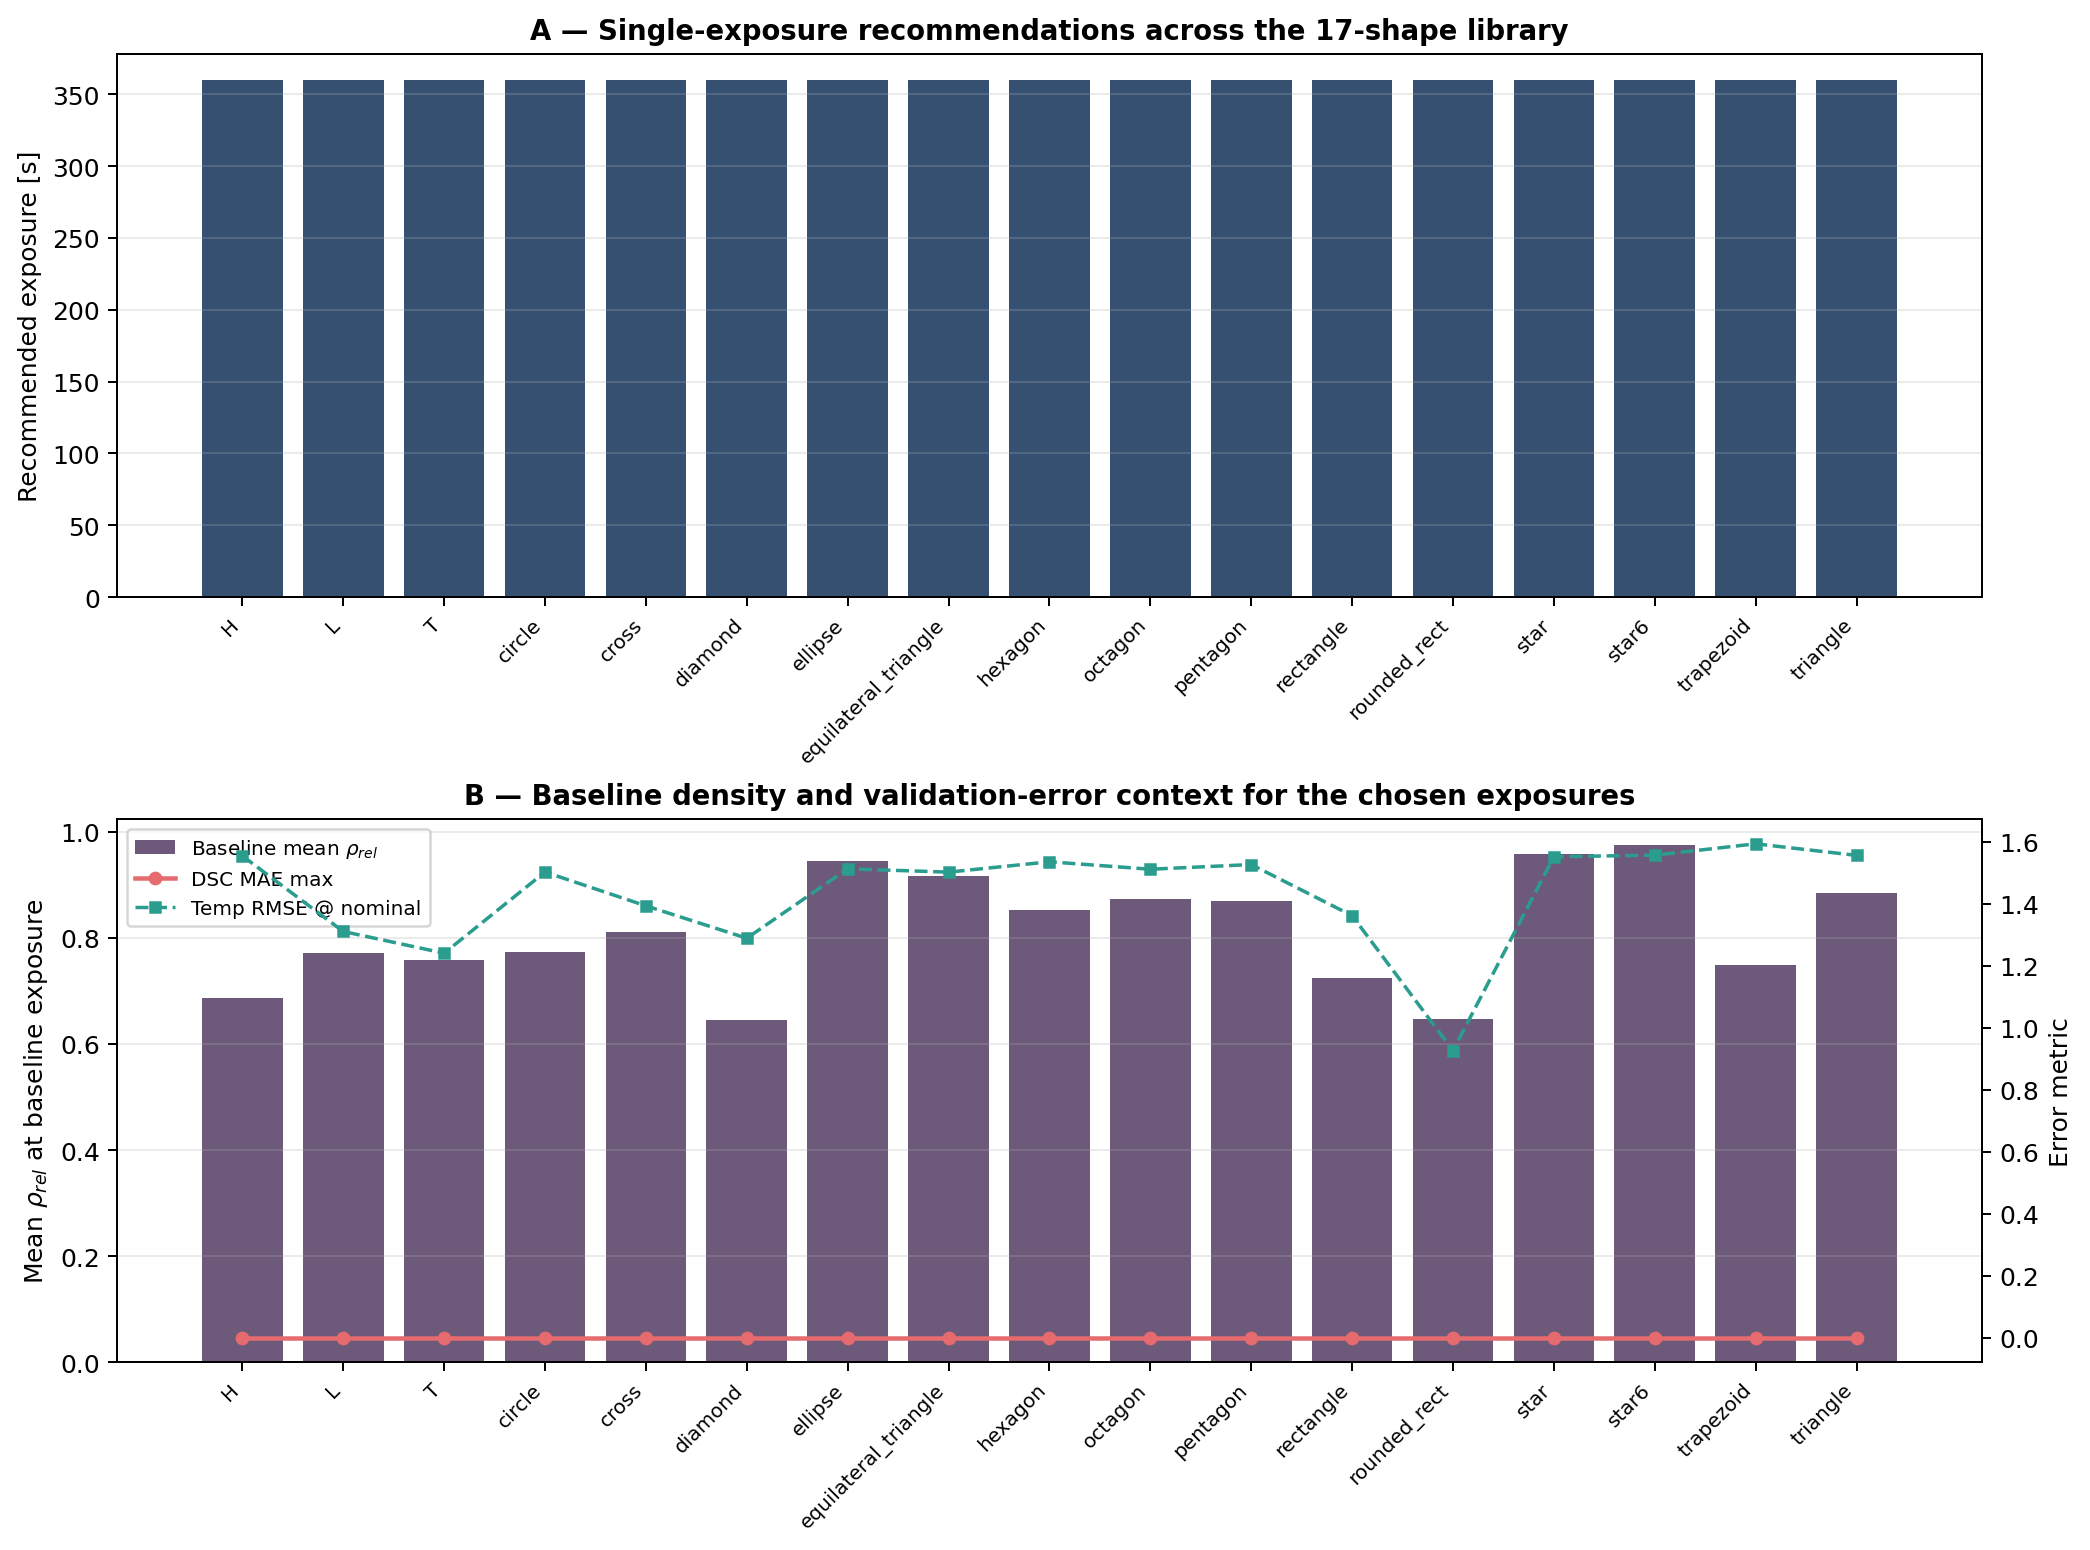
\includegraphics[width=\textwidth]{fig_single_library_refresh.png}
  \caption{Refreshed single-exposure library summary for the 17 retained
           canonical geometries.  Top: recommended exposure from the
           reusable \SIlist{360;420;480}{\second} screening set.
           Bottom: baseline mean relative density together with the
           diagnostic columns now carried into the paper workflow.}
  \label{fig:primitive_sweep}
\end{figure*}

\begin{table*}[tb]
\centering
\caption{Single-exposure summary for the refreshed 17-shape library using the DSC-calibrated PA12 model family. The chosen exposure is the minimum sweep exposure retained in the reusable screening dataset that matched the baseline density target while keeping the diagnostic errors reported for transparency.}
\label{tab:single_library_refresh}
\small
\begin{tabular}{lrrrrrr}
\toprule
Geometry & Exp. [s] & Base. $\phi$ & Base. $\rho_{rel}$ & DSC MAE$_{max}$ & Temp RMSE$_{360}$ [C] & $\rho$ RMSE$_{360}$ \\
\midrule
H & 360 & 0.869 & 0.686 & 0.000 & 1.55 & 0.007 \\
L & 360 & 0.688 & 0.770 & 0.000 & 1.31 & 0.004 \\
T & 360 & 0.600 & 0.758 & 0.000 & 1.24 & 0.004 \\
circle & 360 & 0.874 & 0.773 & 0.000 & 1.50 & 0.008 \\
cross & 360 & 0.734 & 0.812 & 0.000 & 1.39 & 0.004 \\
diamond & 360 & 0.517 & 0.644 & 0.000 & 1.29 & 0.004 \\
ellipse & 360 & 0.997 & 0.944 & 0.000 & 1.51 & 0.004 \\
equilateral_triangle & 360 & 0.992 & 0.916 & 0.000 & 1.50 & 0.004 \\
hexagon & 360 & 0.963 & 0.853 & 0.000 & 1.54 & 0.006 \\
octagon & 360 & 0.990 & 0.873 & 0.000 & 1.51 & 0.005 \\
pentagon & 360 & 0.949 & 0.870 & 0.000 & 1.53 & 0.006 \\
rectangle & 360 & 0.961 & 0.724 & 0.000 & 1.36 & 0.007 \\
rounded_rect & 360 & 0.764 & 0.647 & 0.000 & 0.93 & 0.005 \\
star & 360 & 0.989 & 0.958 & 0.000 & 1.55 & 0.003 \\
star6 & 360 & 1.000 & 0.975 & 0.000 & 1.56 & 0.003 \\
trapezoid & 360 & 0.941 & 0.749 & 0.000 & 1.59 & 0.008 \\
triangle & 360 & 1.000 & 0.884 & 0.000 & 1.56 & 0.007 \\
\bottomrule
\end{tabular}
\end{table*}

\subsection{Effect of Shape Symmetry}

The refreshed screening view preserves the same broad geometric lesson
as the earlier table even though the presentation has changed: geometry
still matters strongly.  Symmetric shapes and smoothly varying
boundaries continue to show different melt and density behavior from
concave or strongly directional shapes, but the updated table now
emphasizes that these trends should be interpreted together with their
error diagnostics instead of as standalone numbers.

In particular, the concave L-, T-, and cross-like families remain
useful stress tests because they expose the shielded, parallel-face
regions that motivate later discussion of turntable averaging and
orientation optimization.

\subsection{The Diamond Paradox}

The diamond (square rotated $45^\circ$) presents an instructive
case: it has the lowest mean temperature of any shape (only
$\SI{179.5}{\celsius}$, barely above the melt threshold) and the
lowest overall density ($\bar{\rhorel} = 0.644$), yet its tip corners
reach extreme temperatures ($T_{\max} \approx \SI{272}{\celsius}$).
The reason is geometric: a diamond oriented at $45^\circ$ presents
all four faces at $45^\circ$ to the applied field.  There is no
purely perpendicular face ($0^\circ$) and no purely parallel face
($90^\circ$); instead, all faces are at intermediate angles where the
effective field enhancement is $\approx 3$--$5\times$ the mean.  While
vertices still have the tip effect, the faces---which constitute the
majority of the boundary---receive field enhancement comparable to the
center rather than the strong normal-field enhancement of the $0^\circ$
faces.  The result is overall lower heating with extreme tip hot-spots
and poor overall densification.

\subsection{Shape Design Implications}

The shape library reveals three practical design guidelines for RFAM:
(a) shapes with many equal-angle vertices distribute field concentration
most uniformly;
(b) concave re-entrant features systematically increase $\bndstd$
regardless of overall shape symmetry (L, T, Cross);
(c) reducing corner sharpness (Rounded rect vs. Rectangle) reduces
$\bndstd$ from 0.106 to 0.105 and increases $r_{\mathrm{bnd}}$ from
0.601 to 0.712, even though the improvement in $\bndstd$ itself is
marginal---the primary benefit is the increase in the worst-case
minimum boundary density.

%% ---------------------------------------------------------------
\FloatBarrier
\section{Geometry Prewarp Results}
\label{sec:results_prewarp}
%% ---------------------------------------------------------------

The prewarp workflow remains important conceptually, but it should be
read here as a reduced-status prototype section.  The currently
reusable prewarp artifacts in this repository are still tied to the
earlier baseline-model workflow rather than to the refreshed
DSC-calibrated PA12 stack used for the main single-exposure, turntable,
and orientation-optimizer comparisons.  Accordingly, the prewarp
results below are retained to document current tool capability and
limitations, not to serve as the primary quantitative result of the
paper.  \Cref{tab:prewarp_refresh} summarizes the reduced legacy
prewarp metrics that are still reproducible from saved artifacts.

\begin{table}[tb]
\centering
\caption{Reduced legacy prewarp summary retained only to document the current prototype status. These runs were generated with the earlier baseline-model workflow and are therefore discussed separately from the refreshed DSC-calibrated result set.}
\label{tab:prewarp_refresh}
\small
\begin{tabular}{lrr}
\toprule
Case & RMSE [mm] & Boundary std \\
\midrule
Circle legacy prewarp & 0.1026 & 0.1105 \\
Square legacy prewarp & 0.1526 & 0.0403 \\
\bottomrule
\end{tabular}
\end{table}

\subsection{$\Leff$ Calibration for Circle and Square}

\Cref{tab:leff_calibration} presents the calibration sweep results
for the circle and square, and \cref{fig:leff_calibration} plots
the full RMSE-vs-$\Leff$ curves for both shapes.  For the circle,
the optimal $\Leff = \SI{5}{\milli\meter}$ achieves
$\RMSE = \SI{0.103}{\milli\meter}$ in 2 iterations.  The circle's
smooth boundary with gradual EPE variation enables the algorithm to
converge reliably to a low RMSE; large $\Leff$ values
($\geq \SI{10}{\milli\meter}$) lead to over-correction oscillations
that prevent convergence within the iteration budget.

For the square, the optimal $\Leff = \SI{7}{\milli\meter}$ achieves
$\RMSE = \SI{0.153}{\milli\meter}$.  The higher optimal $\Leff$ and
residual RMSE compared to the circle reflects the square's sharp corners,
where the EPE changes discontinuously at the $90^\circ$ vertex.  The
prewarp algorithm cannot fully correct these corner singularities
because the shrinkage model (\cref{eq:shrinkage_ratio}) does not capture
the three-dimensional redistribution of material at a sharp corner during
sintering.

\begin{table}[tb]
\centering
\caption{$\Leff$ calibration sweep: post-convergence geometric RMSE
         (\si{\milli\meter}) for circle and square targets.  Bold
         indicates the optimal value selected for each shape.}
\label{tab:leff_calibration}
\begin{tabular}{cSS}
\toprule
$\Leff$ (mm) & {Circle RMSE (mm)} & {Square RMSE (mm)} \\
\midrule
3  & 0.117 & 0.209 \\
\textbf{5}  & \textbf{0.103} & 0.182 \\
7  & 0.194 & \textbf{0.153} \\
10 & 0.167 & 0.174 \\
13 & 0.151 & 0.227 \\
16 & 0.151 & 0.241 \\
\bottomrule
\end{tabular}
\end{table}

\begin{figure}[H]
  \centering
  \begin{subfigure}[b]{\columnwidth}
    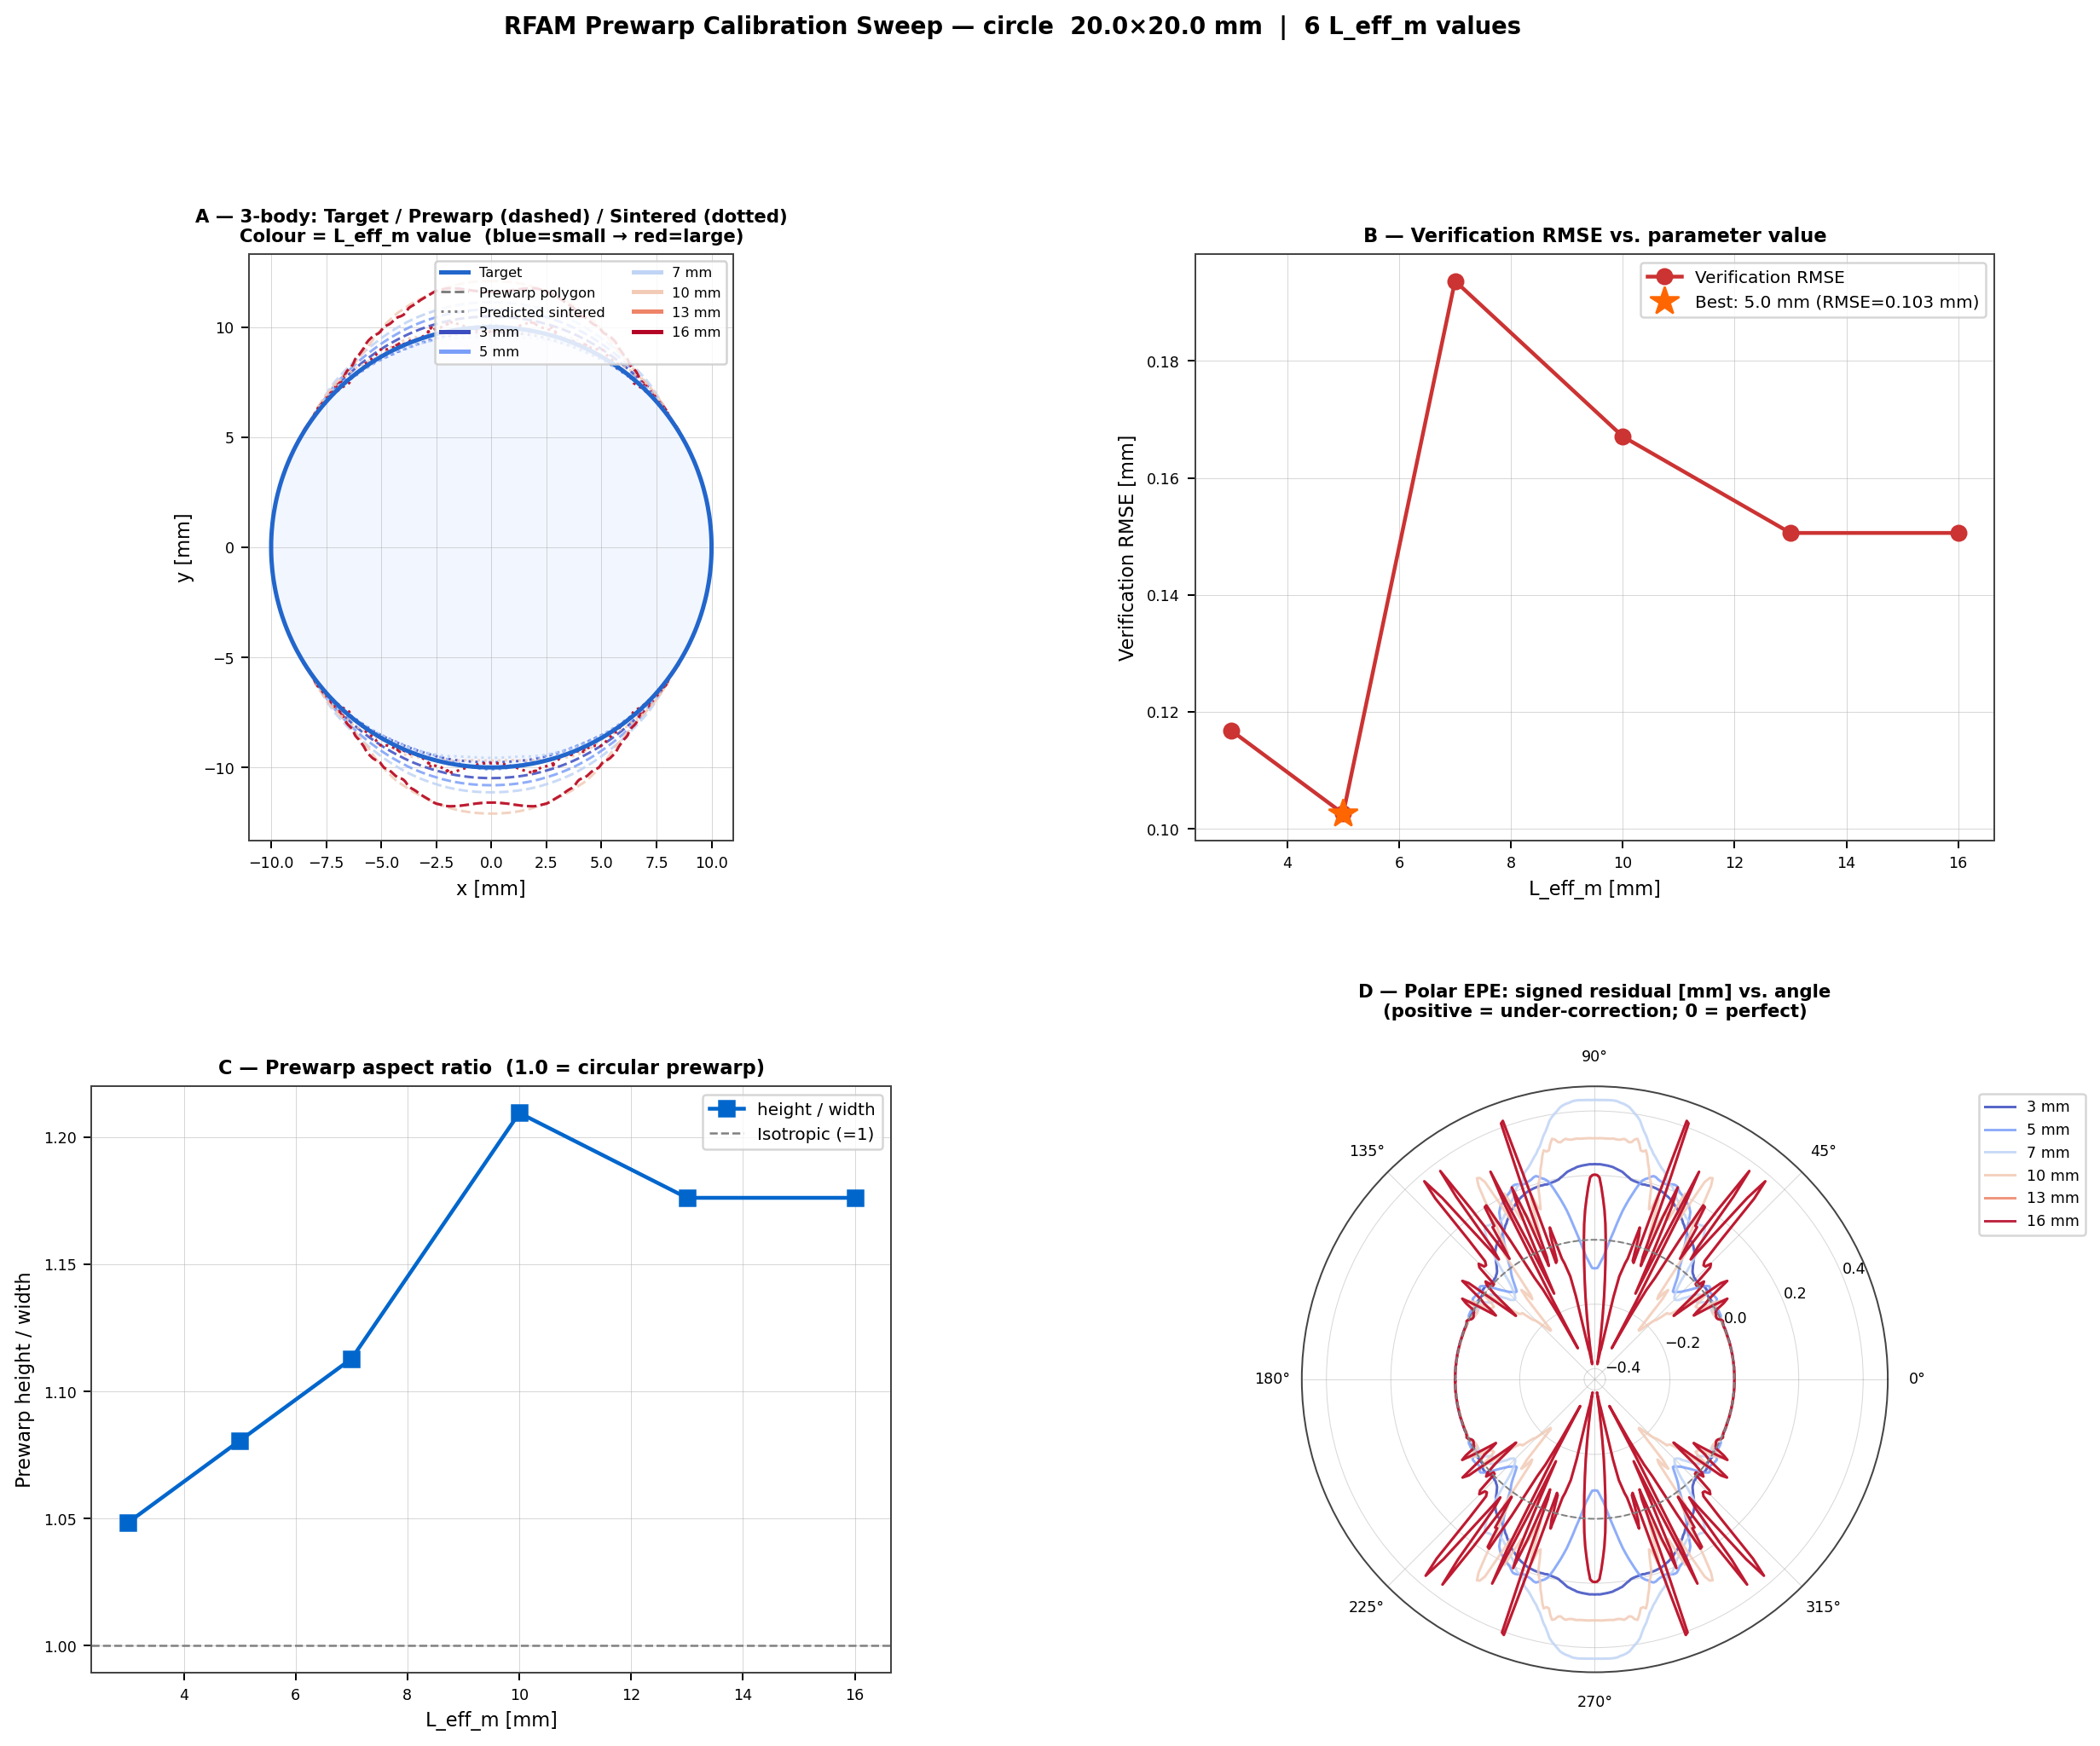
\includegraphics[width=\columnwidth]{fig_calib_circle.png}
    \caption{Circle: $\RMSE$ vs.\ $\Leff$ at convergence.}
    \label{fig:leff_circle}
  \end{subfigure}
  \par\smallskip
  \begin{subfigure}[b]{\columnwidth}
    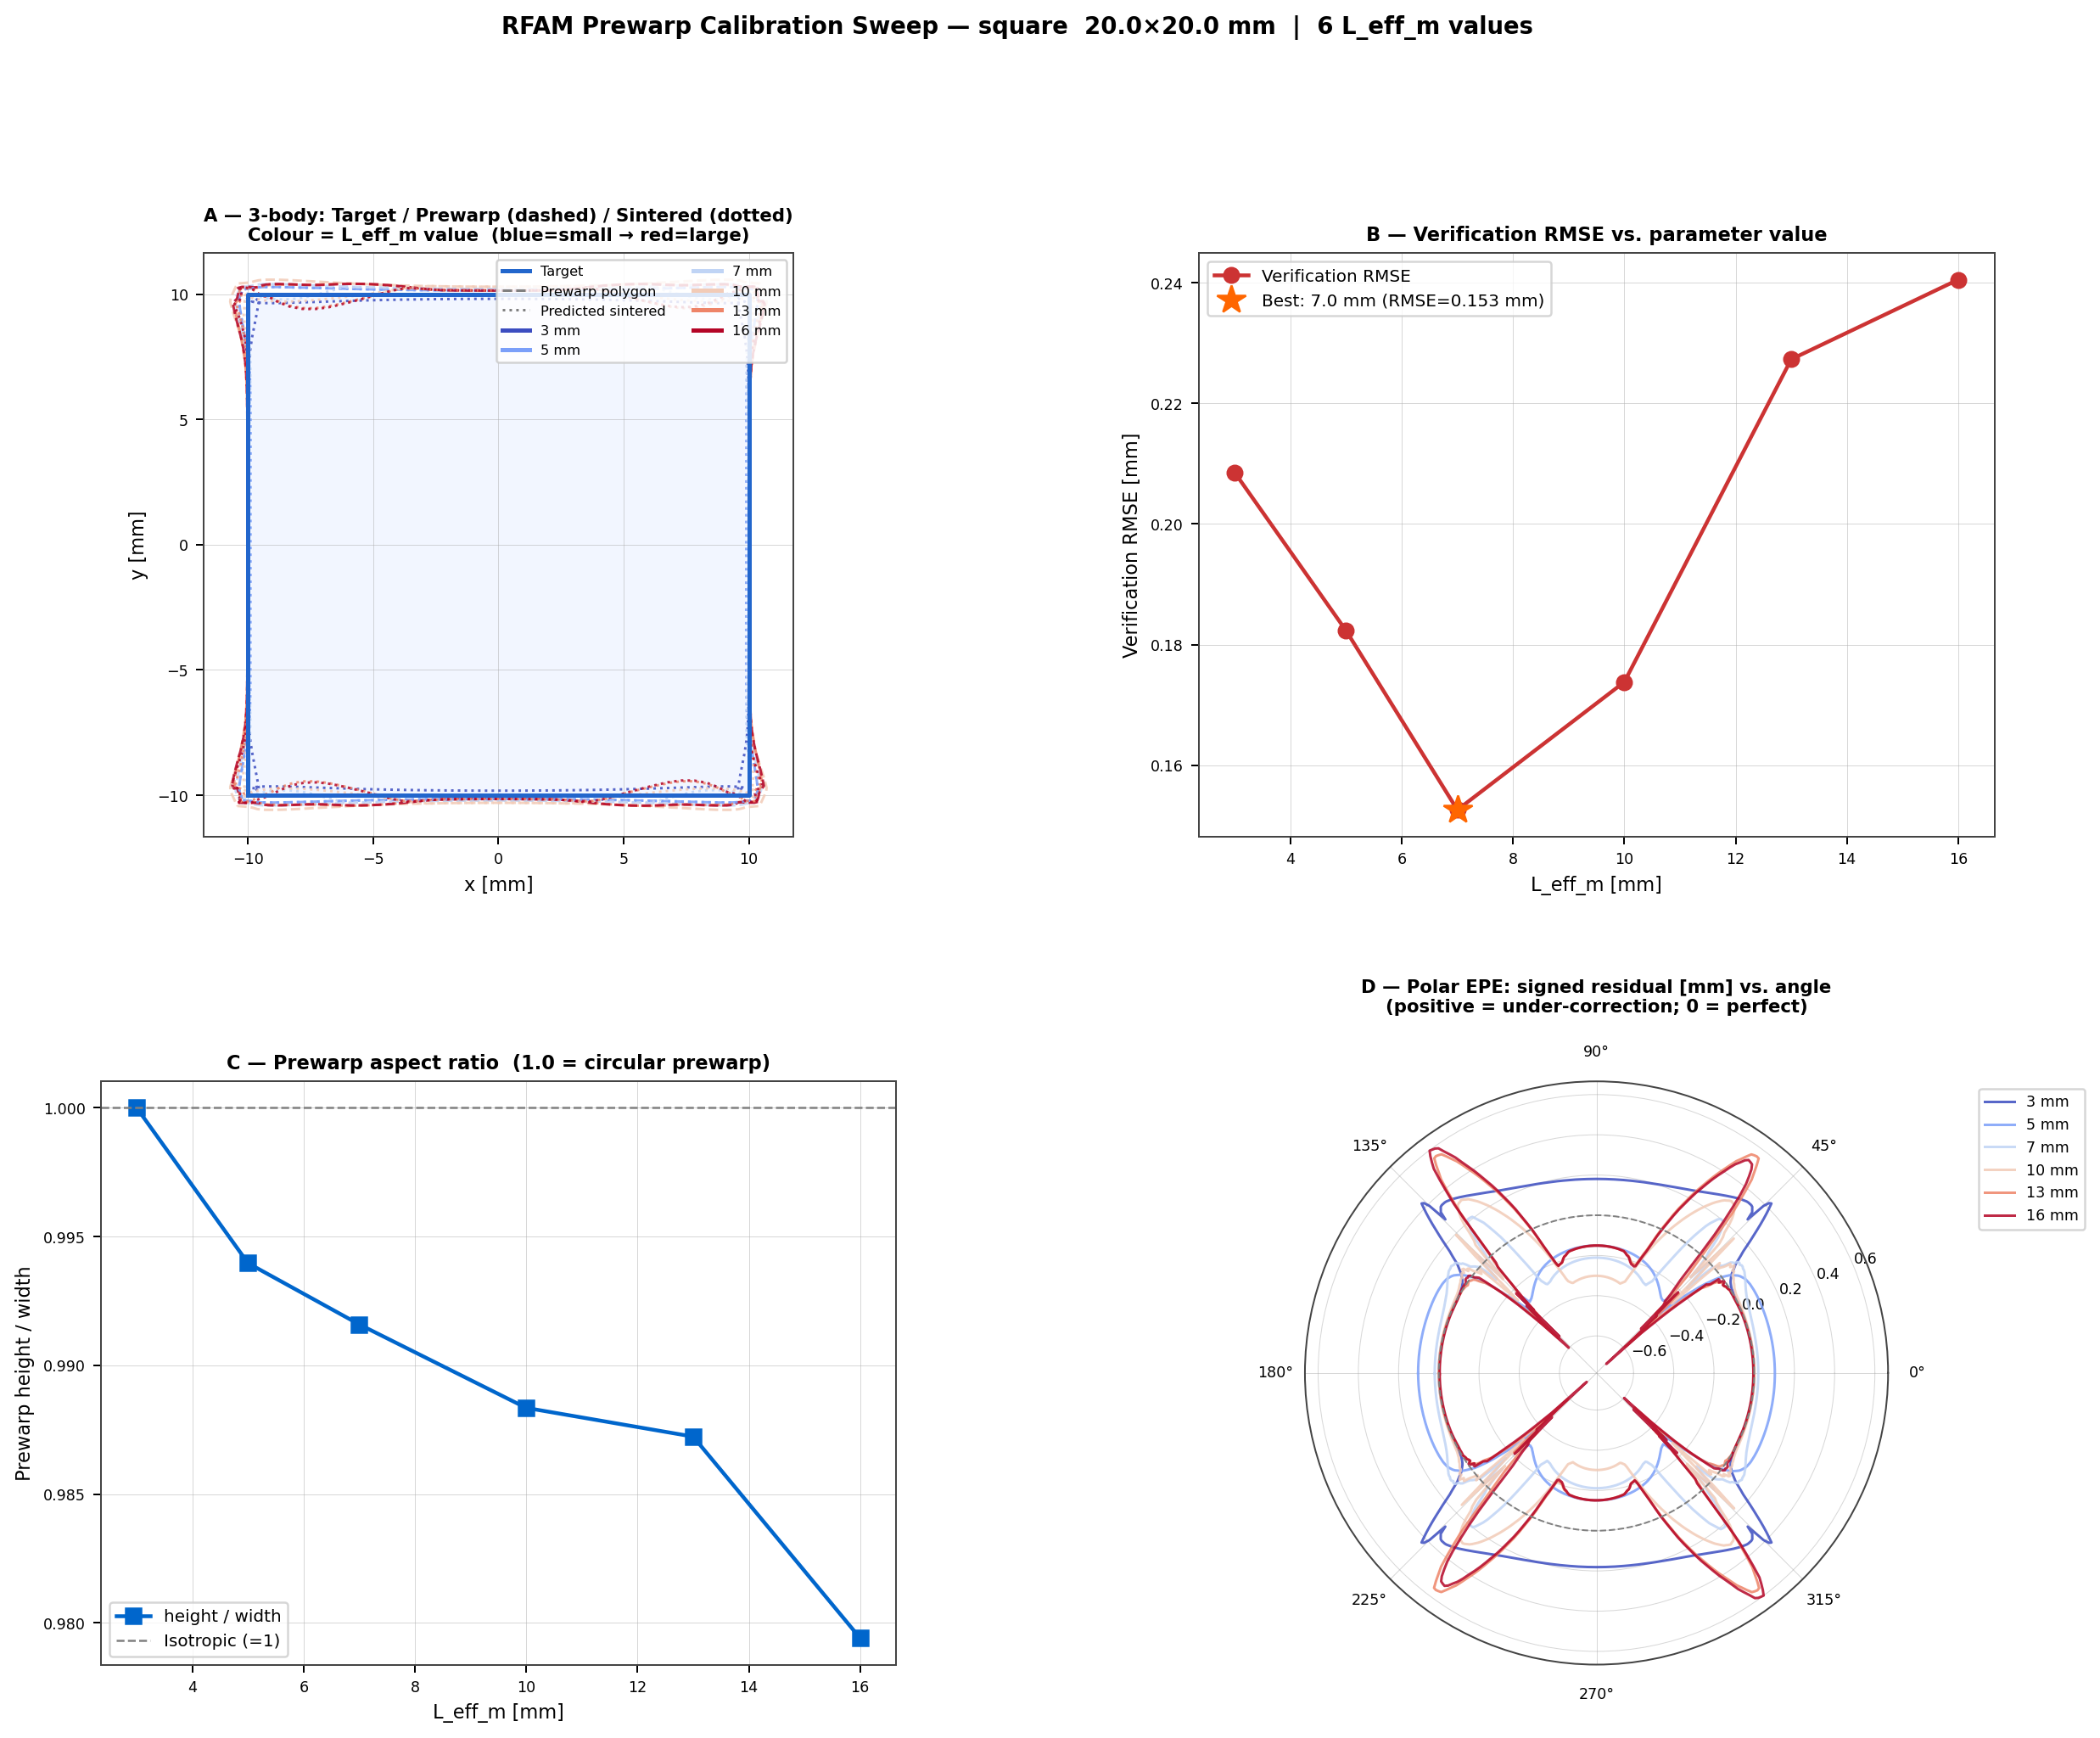
\includegraphics[width=\columnwidth]{fig_calib_square.png}
    \caption{Square: $\RMSE$ vs.\ $\Leff$ at convergence.}
    \label{fig:leff_square}
  \end{subfigure}
  \caption{Effective shrinkage length $\Leff$ calibration sweeps.
           Each point represents the post-convergence RMSE after running
           the full EPE-gradient-descent algorithm.  The optimal values
           are $\Leff = \SI{5}{\milli\meter}$ (circle) and
           $\Leff = \SI{7}{\milli\meter}$ (square).}
  \label{fig:leff_calibration}
\end{figure}

\subsection{Square Prewarp Validation}

\Cref{fig:square_prewarp} shows the prewarp result for the square
target.  The prewarp polygon (input to the simulator) is noticeably
convex: the corners protrude inward relative to a square, and the face
midpoints protrude outward slightly, compensating for the greater
shrinkage at corners vs. face midpoints.  The RMSE improves from
\SI{0.37}{\milli\meter} (uncorrected, iteration 0) to
\SI{0.153}{\milli\meter} (converged, iteration 2), a 59\% reduction.

The boundary density after prewarp is also improved: the prewarp polygon
forces the parallel-face midpoints to extend further outward, increasing
the local field coupling at those previously under-heated regions.  This
geometric effect reduces $\bndstd$ from 0.072 (unprewarped) to 0.040
(prewarped), a 44\% reduction---a genuine side benefit of the prewarp
in addition to its intended geometric correction.

\begin{figure}[H]
  \centering
  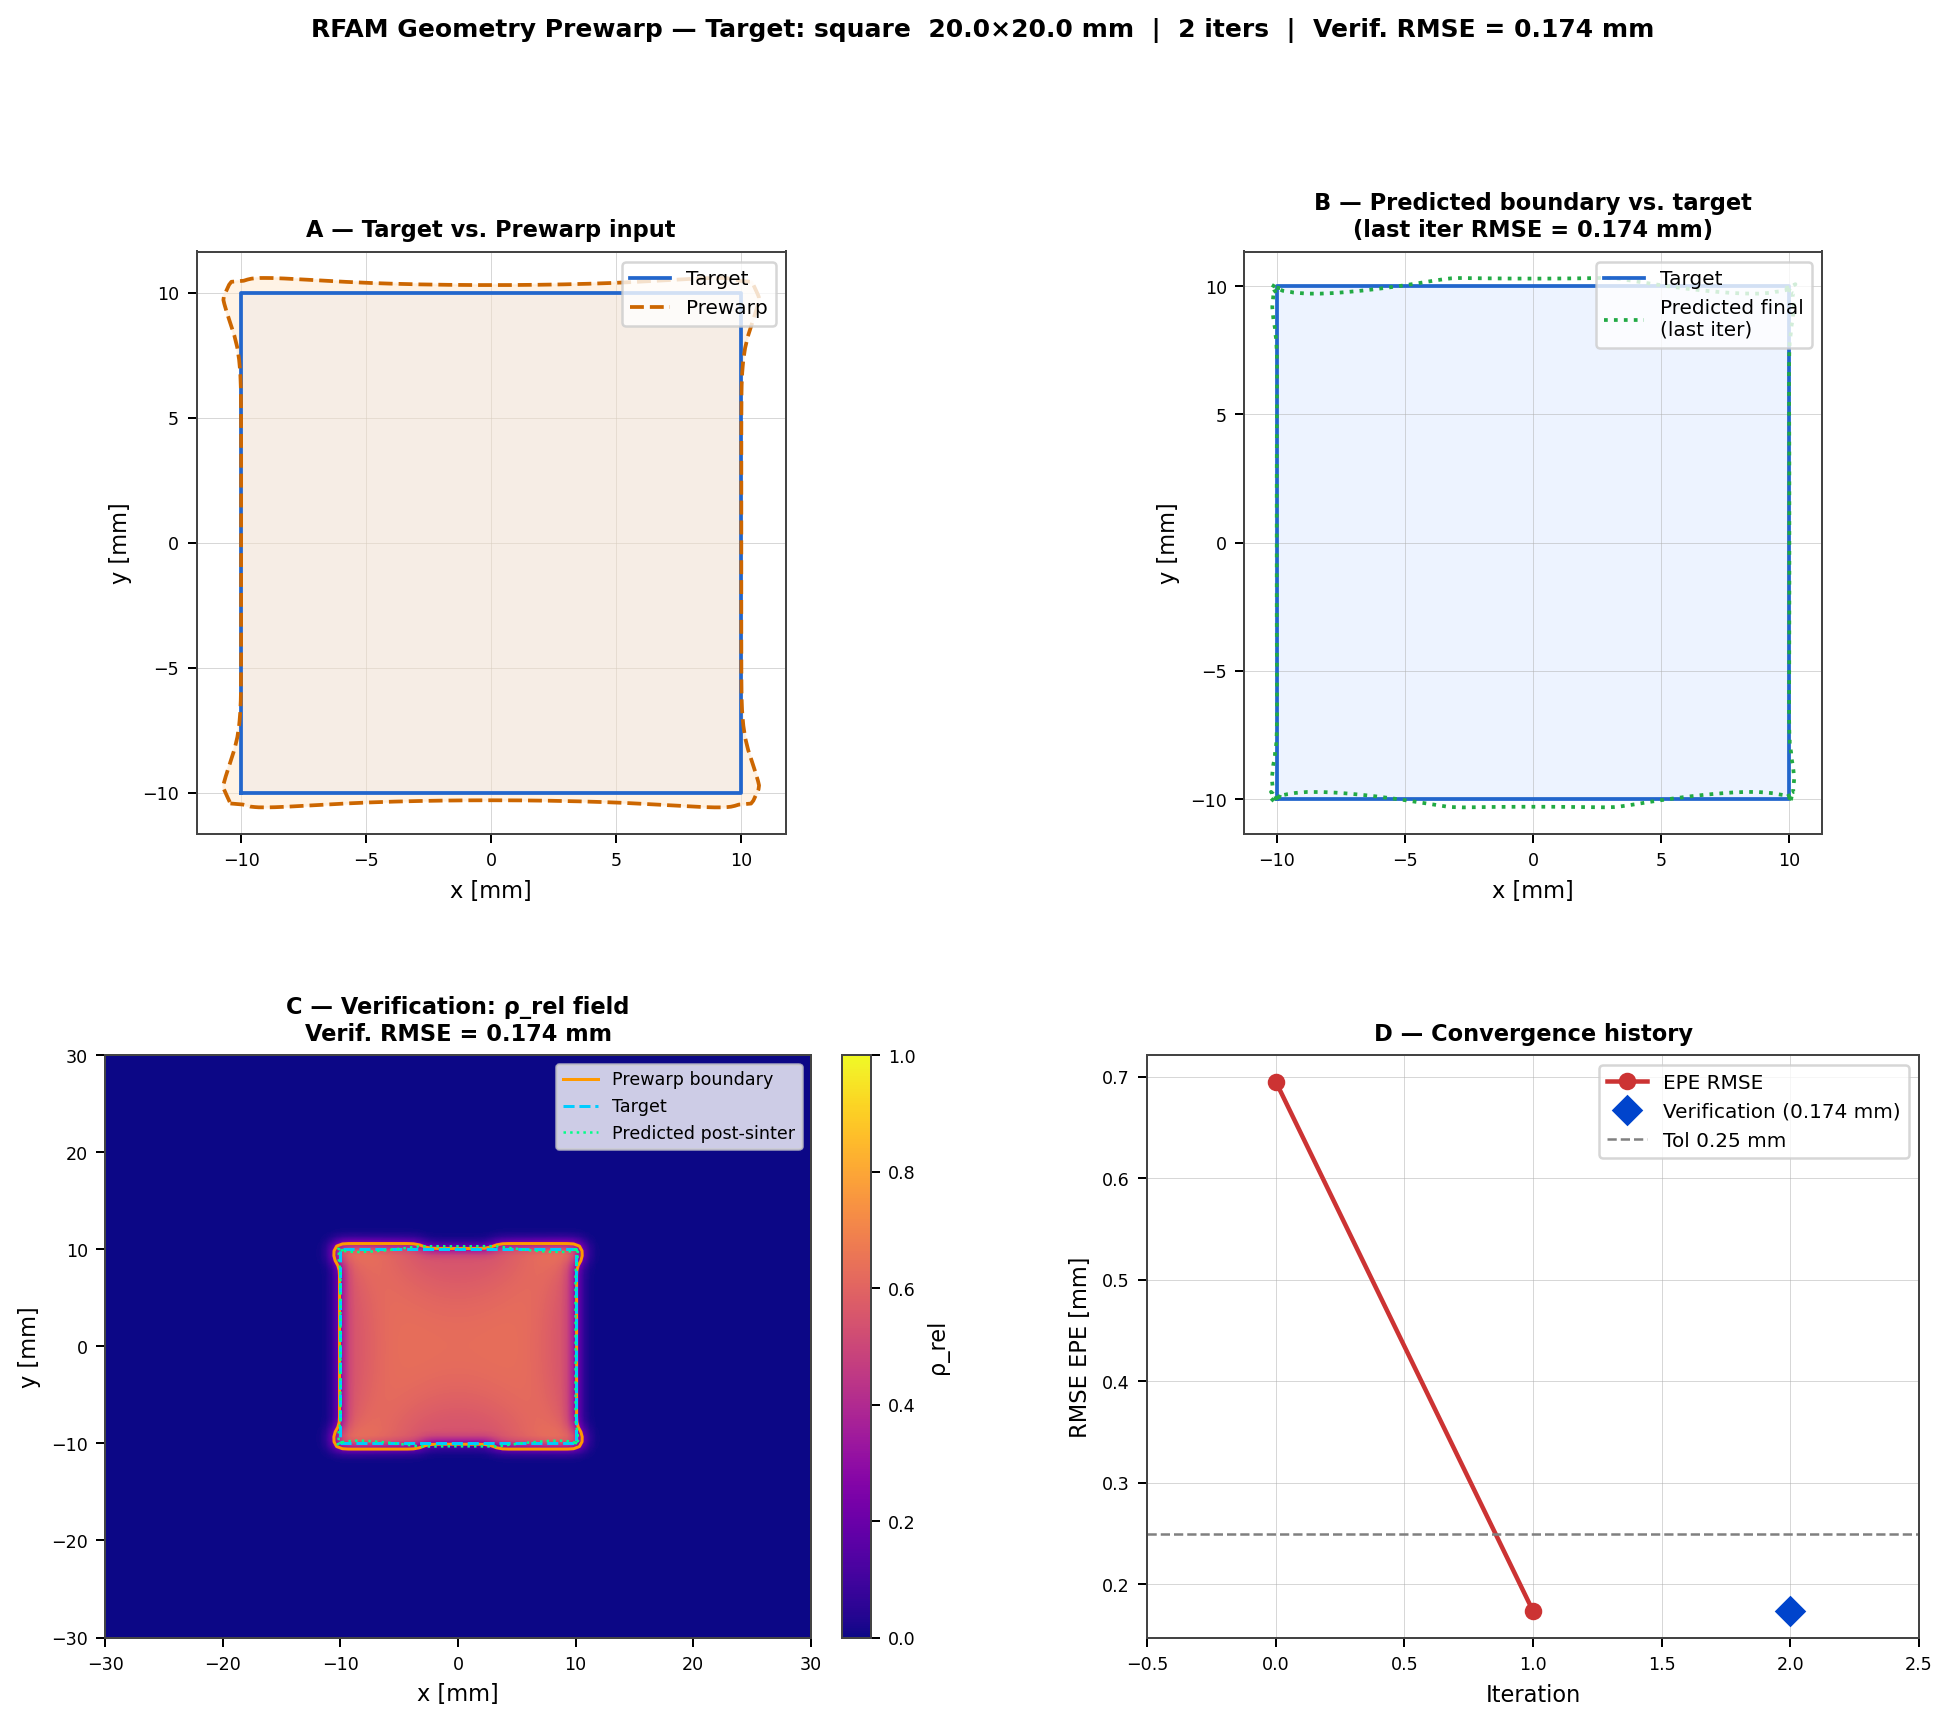
\includegraphics[width=\columnwidth]{fig_prewarp_square.png}
  \caption{Square prewarp result using $\Leff = \SI{7}{\milli\meter}$.
           Top: prewarp polygon (blue) vs.\ target (dashed red).
           Bottom: predicted sintered boundary (green) vs.\ target.
           RMSE reduces from \SI{0.37}{\milli\meter} (unprewarped) to
           \SI{0.153}{\milli\meter} after 2 iterations.}
  \label{fig:square_prewarp}
\end{figure}

\subsection{H-Shape Prewarp}
\label{sec:hshape_prewarp}

The H-shape presents a substantially more challenging prewarp problem.
Its bounding box is $20 \times \SI{20}{\milli\meter}$ with two vertical
legs (\SI{6}{\milli\meter} wide) connected by a horizontal crossbar
(\SI{6}{\milli\meter} tall, spanning between the legs at mid-height).
The shape has 5 geometrically distinct face categories:
\begin{enumerate}
  \item Outer vertical legs (parallel to $\vect{E}$, under-heated):
        $\rhorel^{\mathrm{bnd}} \approx 0.610$ at midpoints, as low
        as 0.552 at worst cells
  \item Outer top/bottom faces (perpendicular to $\vect{E}$,
        better-heated): $\rhorel^{\mathrm{bnd}} \approx 0.729$
  \item Crossbar top/bottom faces (perpendicular, partially shielded
        by the legs): $\rhorel^{\mathrm{bnd}} \approx 0.632$
  \item Inner notch faces (parallel, further shielded): $\rhorel \approx 0.679$
  \item Concave inside corners (locally over-heated but inaccessible
        to field from outside due to the notch geometry)
\end{enumerate}

Without correction, $\RMSE = \SI{0.682}{\milli\meter}$ and
$\bndstd = 0.078$.  After 2 prewarp iterations with
$\Leff = \SI{7}{\milli\meter}$, the RMSE decreases to
\SI{0.221}{\milli\meter} (68\% reduction) and $\bndstd$ decreases
to 0.056 (28\% reduction).  The prewarp polygon expands to a bounding
box of $21.00 \times \SI{20.90}{\milli\meter}$, approximately 5\%
larger than the target in each dimension.

\Cref{fig:hshape_prewarp} shows the H-shape prewarp result.  The
non-symmetric expansion is clearly visible: the outer vertical leg
faces protrude more than the horizontal faces, correctly anticipating
the greater shrinkage at those under-heated locations.

\begin{figure}[H]
  \centering
  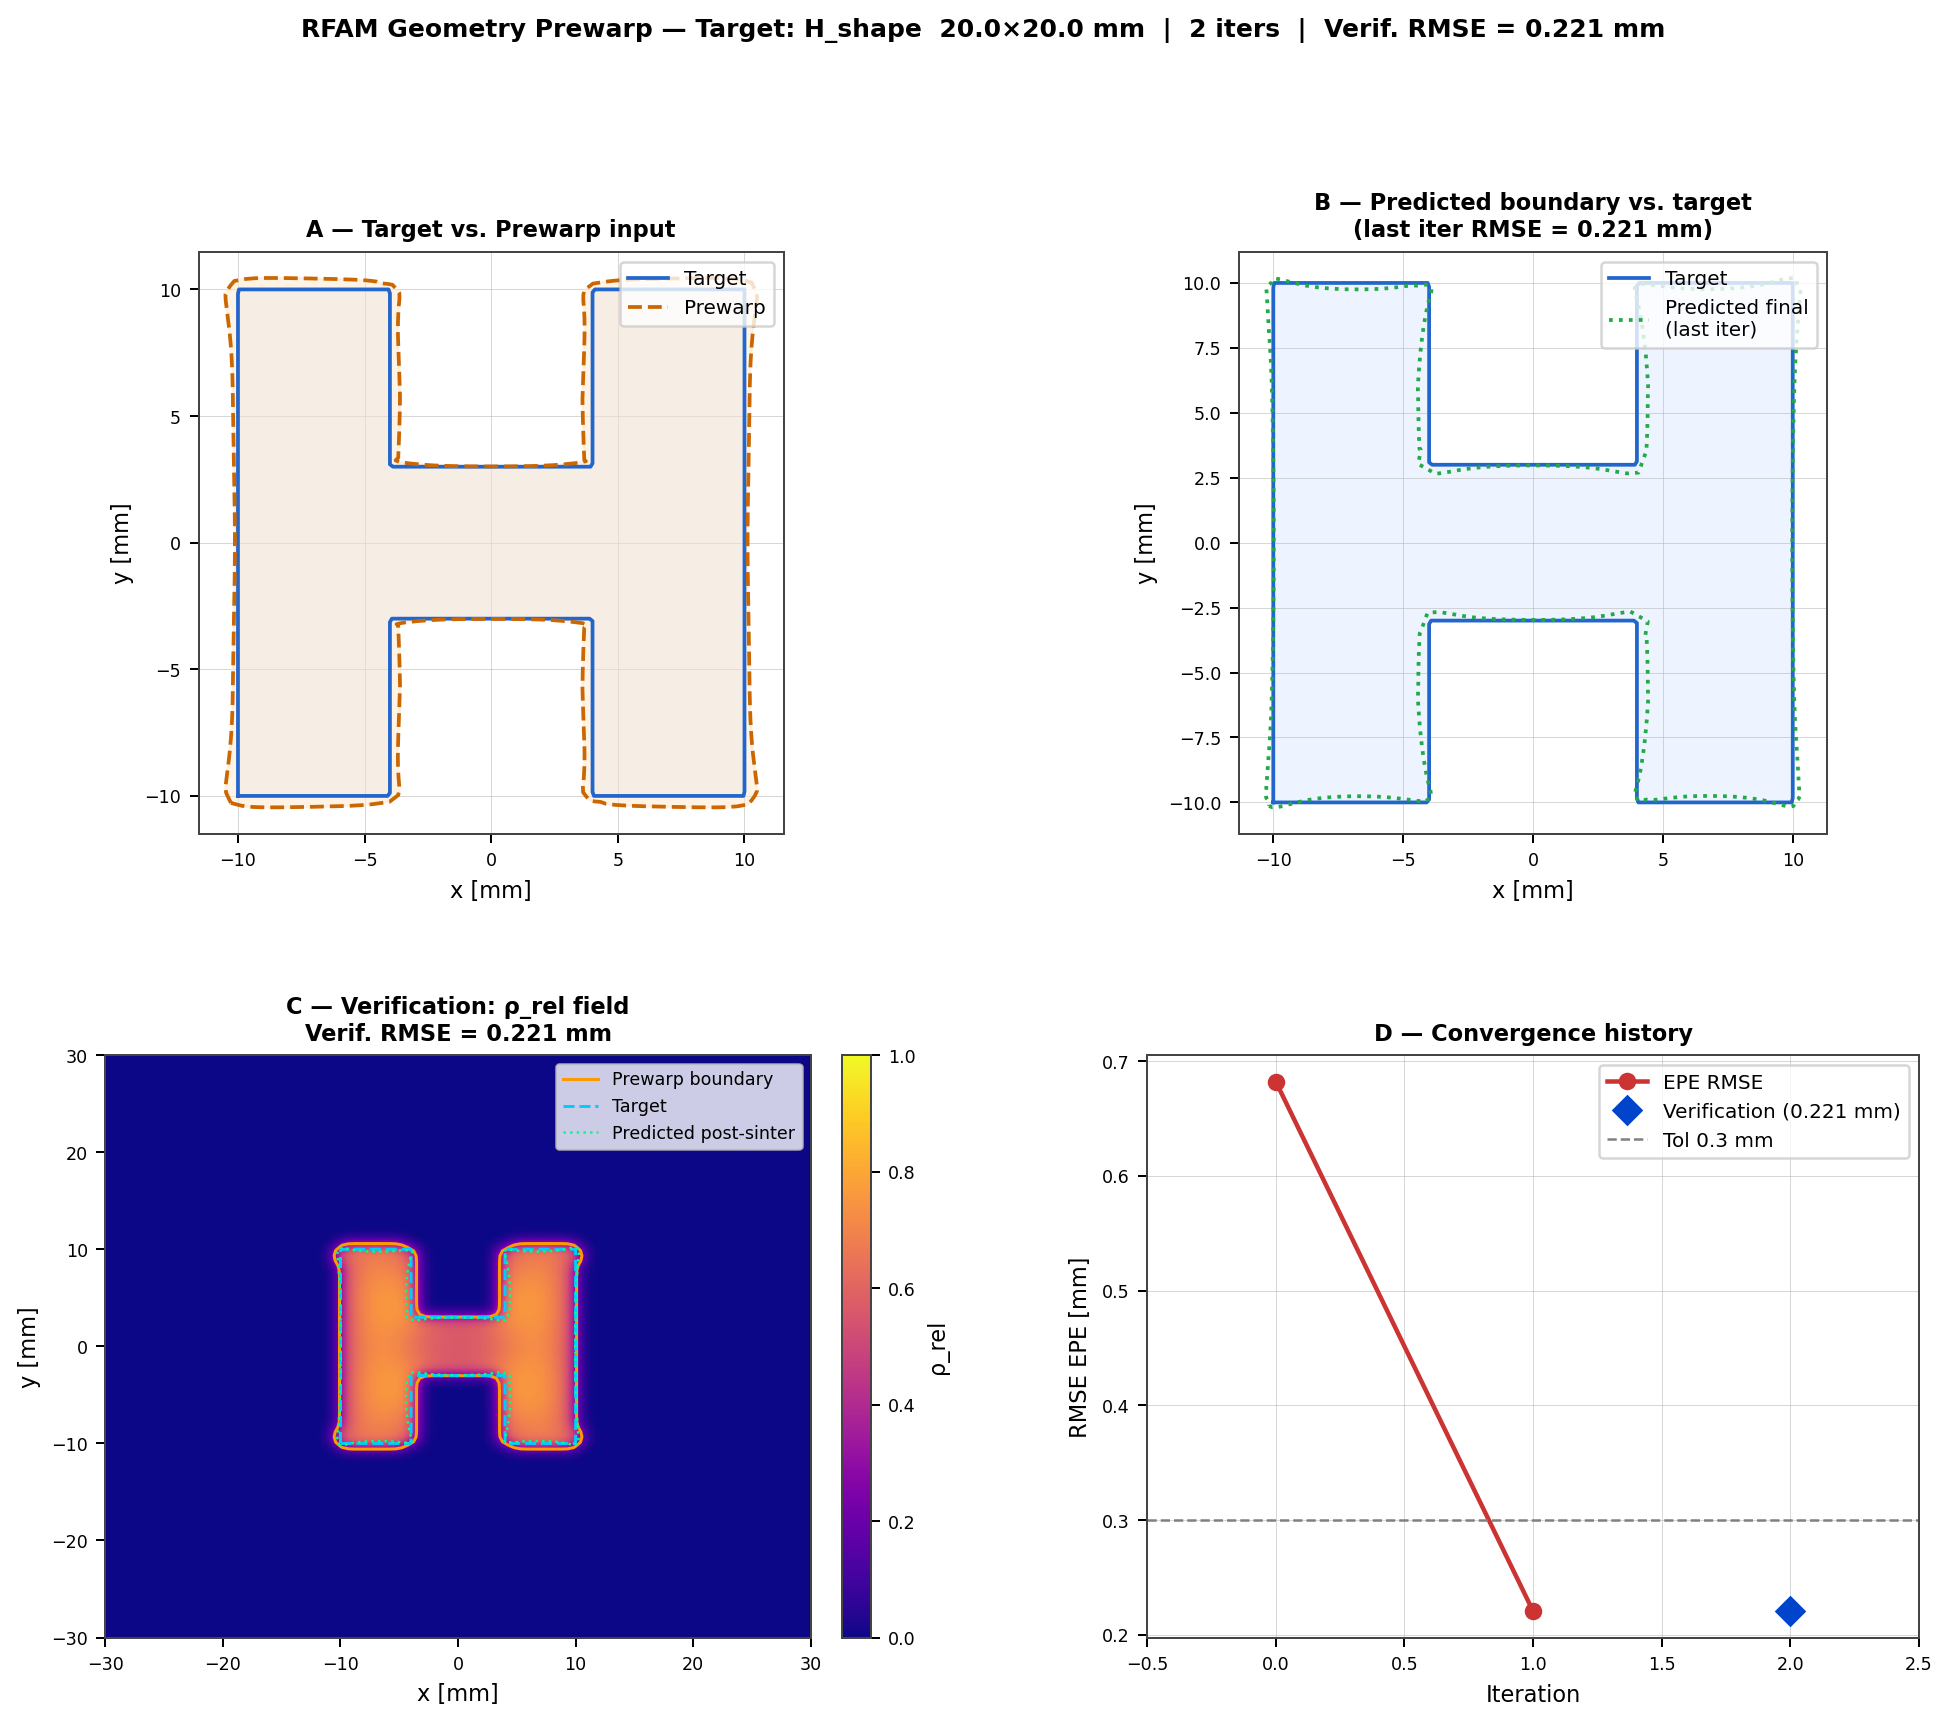
\includegraphics[width=\columnwidth]{fig_prewarp_H.png}
  \caption{H-shape prewarp result ($\Leff = \SI{7}{\milli\meter}$).
           The prewarp polygon (blue) is asymmetrically expanded relative
           to the target (dashed red), with larger expansion at the
           parallel-to-$\vect{E}$ vertical leg faces that would otherwise
           under-sinter and shrink less than expected.  RMSE: 0.682
           (no correction) $\to$ \SI{0.221}{\milli\meter} after
           2 iterations.}
  \label{fig:hshape_prewarp}
\end{figure}

%% ---------------------------------------------------------------
\FloatBarrier
\section{Antennae Energy Concentrators}
\label{sec:results_spikes}
%% ---------------------------------------------------------------

The legacy protrusion-assist terminology is replaced here with
\emph{antennae energy concentrators}, which better reflects the present
RFAM interpretation: small added conductive protrusions intended to
pull field energy toward under-heated faces.  The repository currently
contains only a limited square-study calibration set for this idea, so
this section is now framed as exploratory rather than as a mature
result comparable to the refreshed single-exposure or turntable
sections.

\begin{table}[tb]
\centering
\caption{Antennae energy concentrator snapshot retained as a limited-result section. The current repository only contains a small square-study calibration set, so the refreshed manuscript treats these results as preliminary rather than as a mature design-of-experiments campaign.}
\label{tab:antennae_refresh}
\small
\begin{tabular}{lr}
\toprule
Metric & Value \\
\midrule
Best candidate id & 2 \\
Global antenna size [mm] & 1.5 \\
Square baseline boundary std & 0.0697 \\
Antennae case boundary std & 0.0712 \\
Boundary-std change [\%] & -2.1 \\
Mean $\rho_{rel}$ & 0.605 \\
\bottomrule
\end{tabular}
\end{table}

\begin{figure}[H]
  \centering
  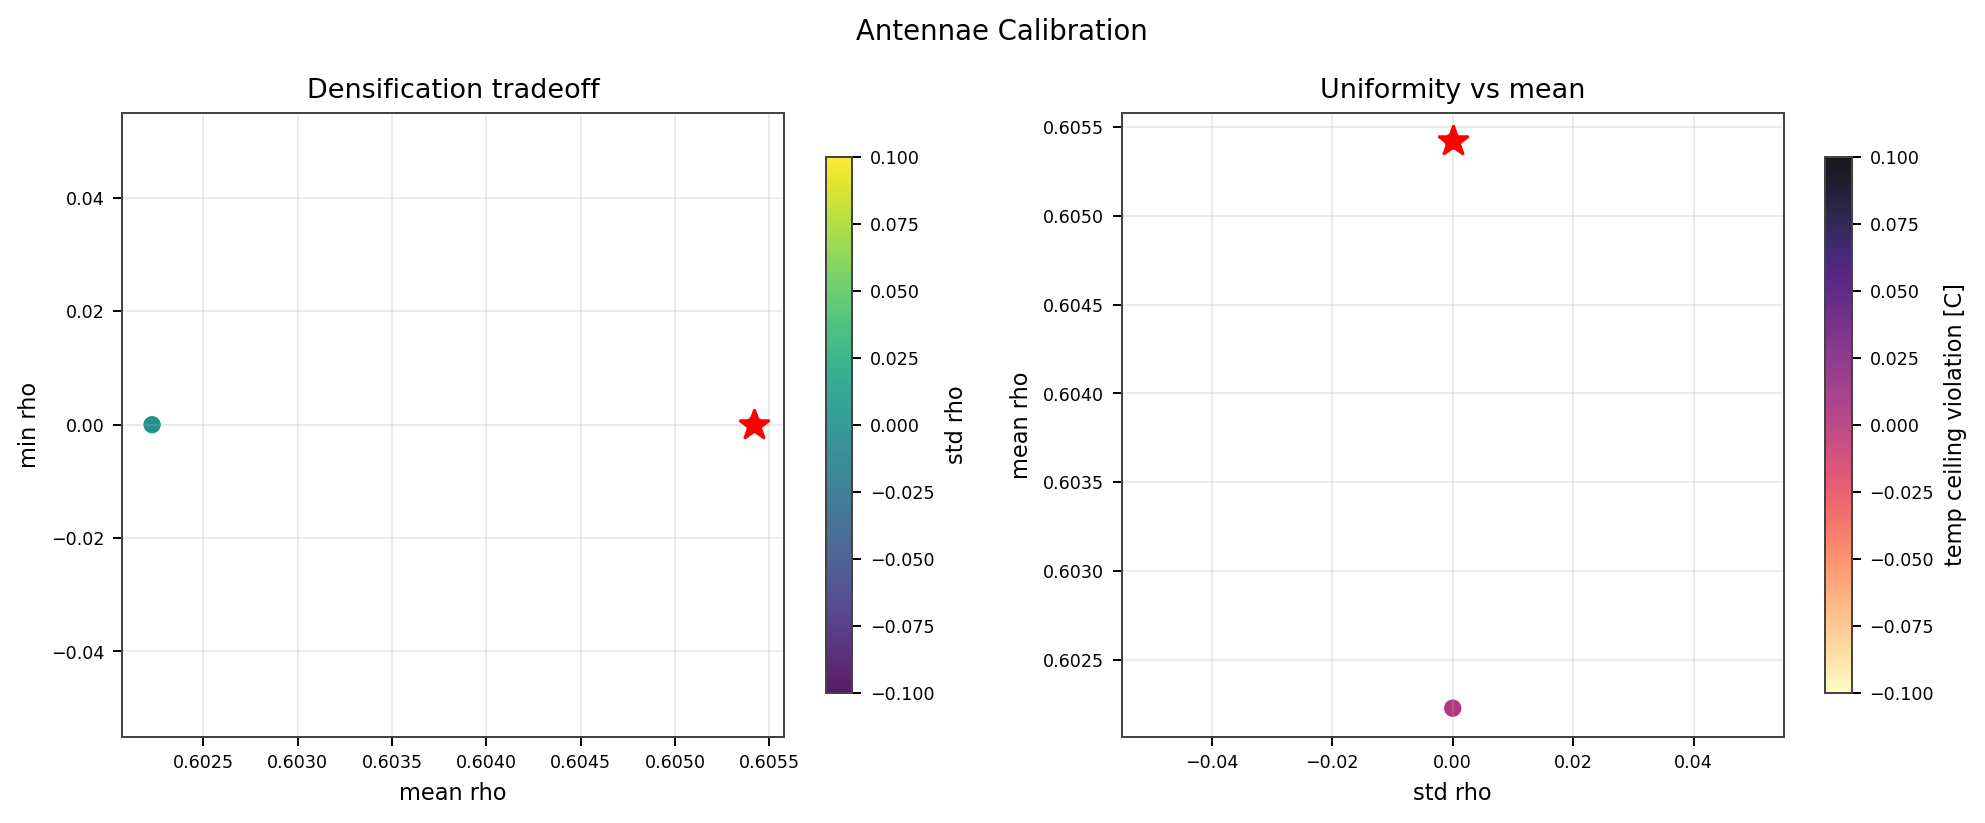
\includegraphics[width=\columnwidth]{fig_antennae_refresh.png}
  \caption{Current antennae energy concentrator calibration artifact.
           The presently reusable square-only calibration set is useful
           for illustrating the concept, but it does not yet support a
           compelling improvement claim: the best retained candidate in
           the current study does not improve the square boundary-density
           standard deviation relative to the plain refreshed baseline.}
  \label{fig:spike_coopt}
\end{figure}

Antennae energy concentrators remain interesting as a future DOE topic,
but the current paper should not overstate their maturity.  Three
limitations remain central:

\paragraph{Limited spatial reach.}
Each $10^\circ$ antenna covers approximately 2 boundary cells on a
$120\times120$ grid.  The 160-cell square perimeter therefore has
only $\approx 2.5\%$ of its boundary cells directly affected by each
antenna.  The concentration effect at the tip does not diffuse
meaningfully to neighboring face cells within the $\SI{360}{\second}$
exposure time.

\paragraph{Geometric impracticality.}
At the sizes explored so far, the added protrusion would clearly print
as a real geometric feature.
An SRAF in optical lithography is deliberately below the resist
resolution threshold; no such threshold exists for RFAM, where any
conductive feature will sinter.  A protrusion of this height would appear
as a $\SI{8}{\milli\meter}$-tall antenna on the finished
part---unacceptable for any functional application.

The conclusion at present is therefore narrower than in the older
draft: antennae energy concentrators are still exploratory.  A proper
design-of-experiments study over size, shape, placement, and count is
still needed before they can be treated as a viable RFAM correction
strategy.

%% ---------------------------------------------------------------
\FloatBarrier
\section{Turntable Rotation Strategy}
\label{sec:results_turntable}
%% ---------------------------------------------------------------

\subsection{Physical Mechanism}

Rotating the part $90^\circ$ converts the two parallel-to-$\vect{E}$
faces into perpendicular-to-$\vect{E}$ faces and vice versa.  With
four $90^\circ$ rotations, each face spends equal time in both
orientations.  In the limit of many infinitesimal rotations, the
exposure would be perfectly uniform (azimuthally averaged field), but
any finite number of discrete rotations retains some residual anisotropy.

The time-based schedule (\cref{eq:rotation_schedule}) distributes
rotations uniformly throughout the exposure.  A single rotation at
$t = \SI{180}{\second}$ (midpoint) would allow the first three minutes
of exposure at one orientation to dominate, while the second three
minutes at the rotated orientation merely attenuate the existing
non-uniformity partially.  By contrast, four rotations at 72 s
intervals ensure that no single orientation dominates: each of the
four $90^\circ$ orientations is active for exactly $\SI{72}{\second}$,
\textit{and} each rotation occurs before significant melting has
occurred (since $T$ only approaches $\Tpc$ near the end of the
exposure for the 6-minute schedule).

\subsection{Results}

\Cref{tab:turntable_core_refresh} presents the refreshed benchmark set.
The current reusable repository artifacts are not perfectly uniform in
schedule across all shapes, so the table now reports the actual
discrete schedule used by each retained run rather than implying that
all cases share the same $4\times 90^\circ$ sequence.

\begin{table*}[tb]
\centering
\caption{Turntable benchmark set for the refreshed manuscript. Boundary metrics were recomputed from the saved fields. The schedules reported here match the reusable run artifacts currently available in the repository, so the exposure durations and discrete rotation sequences are geometry specific.}
\label{tab:turntable_core_refresh}
\small
\begin{tabular}{lcrrrrrr}
\toprule
Geometry & Exp. [s] & Schedule & Single std & Turntable std & Single min/max & Turntable min/max & Turntable residual [\%] \\
\midrule
Square & 360 & 16x45deg over 360 s & 0.0697 & 0.0640 & 0.702 & 0.693 & 0.44 \\
Circle & 360 & 24x30deg over 360 s & 0.1639 & 0.0076 & 0.559 & 0.957 & 63.09 \\
Equilateral triangle & 360 & 16x45deg over 360 s & 0.1582 & 0.0581 & 0.555 & 0.824 & 36.59 \\
L-shape & 720 & 16x45deg over 720 s & 0.1664 & 0.0450 & 0.550 & 0.790 & 27.32 \\
\bottomrule
\end{tabular}
\end{table*}

The refreshed benchmark makes two points.  First, discrete rotation can
still reduce boundary-density anisotropy substantially, especially for
the circle, equilateral triangle, and L-shape.  Second, the new error
columns matter: several of the retained turntable artifacts carry
non-negligible energy-balance residuals, so these should be read as
benchmark-quality comparative runs rather than as final process-design
recommendations.

\begin{figure*}[!t]
  \centering
  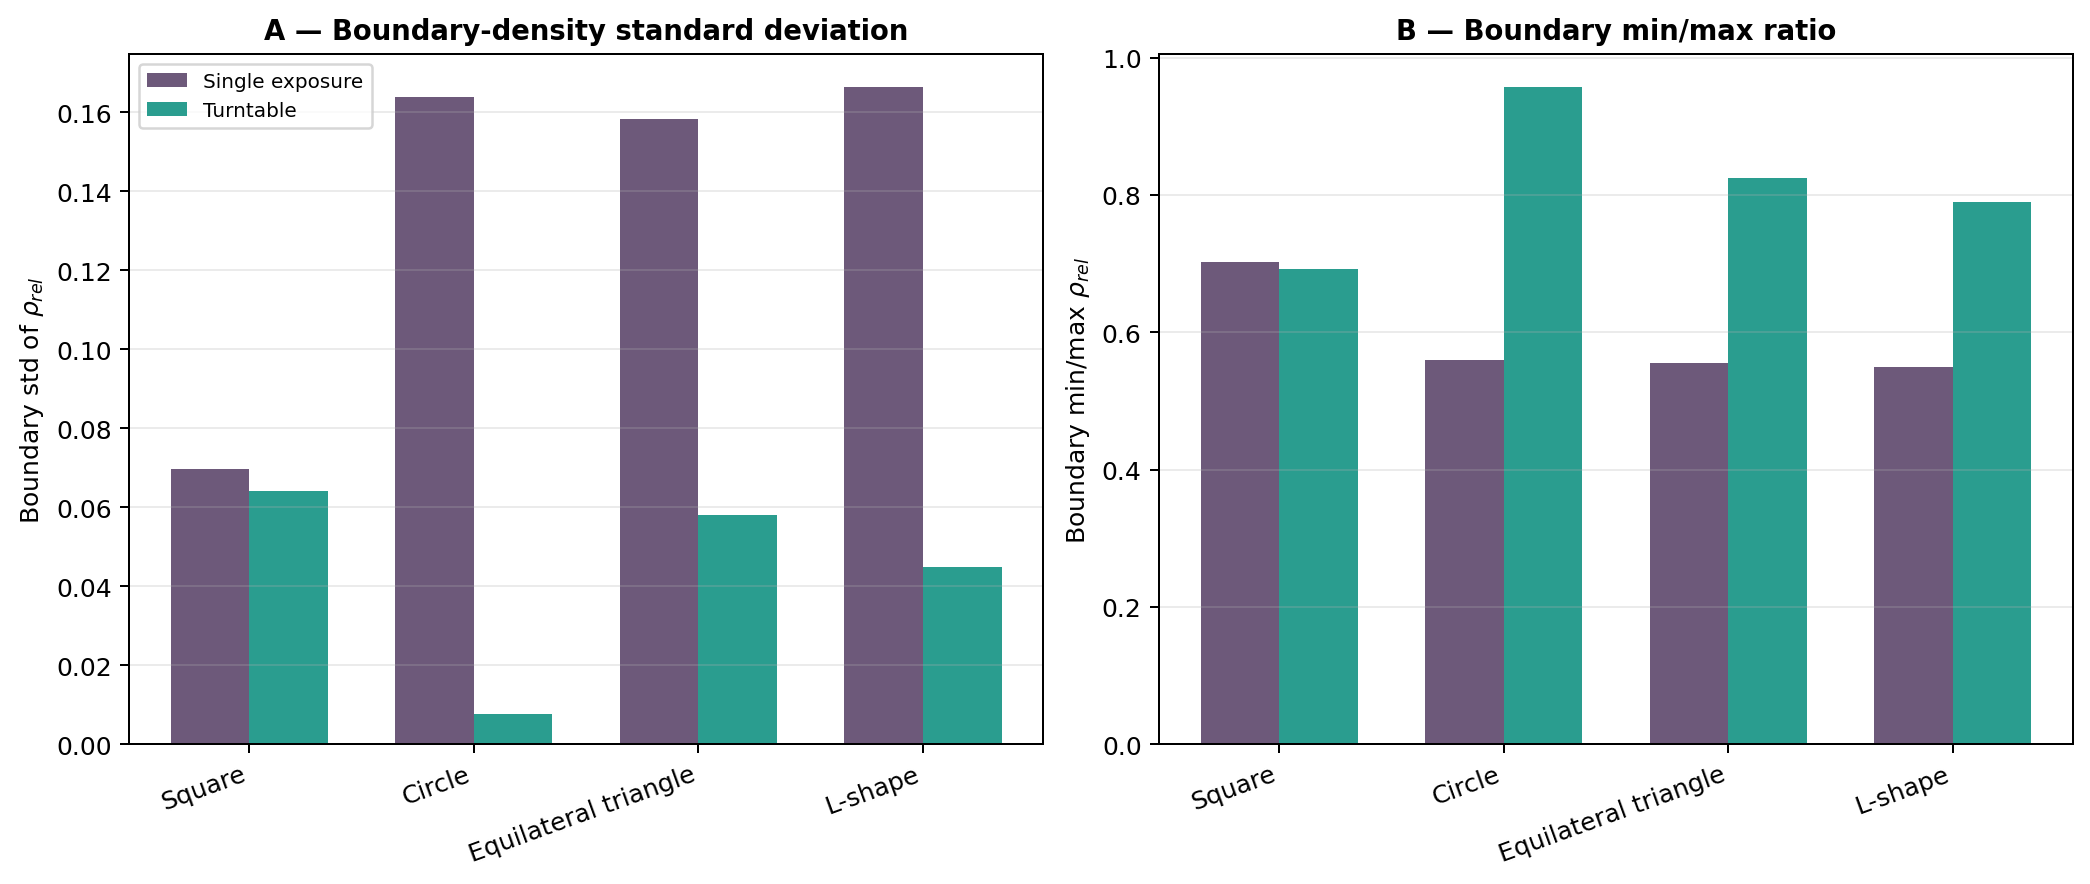
\includegraphics[width=\textwidth]{fig_turntable_core_refresh.png}
  \caption{Refreshed turntable benchmark set generated from reusable
           March~2026 artifacts.  Boundary-density standard deviation and
           min/max ratio were recomputed directly from the saved fields
           for square, circle, equilateral triangle, and L-shape
           comparisons.}
  \label{fig:uniformity_comparison}
\end{figure*}

\Cref{fig:uniformity_comparison} therefore replaces the older
single-square comparison as the paper's main turntable figure.  It
connects more directly to the central question of this refresh: how the
current solver responds across multiple geometries, not just how one
legacy square workflow behaved.

%% ---------------------------------------------------------------
\FloatBarrier
\section{H-Shape: Combined Prewarp and Turntable}
\label{sec:results_combined}
%% ---------------------------------------------------------------

\subsection{H-Shape Baseline and Prewarp}

The H-shape is selected as the primary complex validation case for the
following reasons: (1) it is topologically non-trivial with an internal
cutout; (2) it has 5 geometrically distinct face types with different
electromagnetic coupling; and (3) it is non-symmetric with respect to
the $\vect{E}$-field direction (one axis of symmetry parallel to
$\vect{E}$, one perpendicular).

Because the currently reusable H-shape combined-correction artifacts are
still tied to the older prewarp-centered workflow, this section is best
read as a legacy case study that motivated the present tool
development.  It is retained because the mechanism discussion is still
useful, but the refreshed mainline evidence of this paper now comes
from the 17-shape screening dataset, the turntable benchmark set, and
the orientation-optimizer showcase.

\Cref{tab:hshape_comparison} presents the progressive improvement
from baseline through combined correction.  Without any correction,
the H-shape has $\bndstd = 0.078$ and $r_{\mathrm{bnd}} = 0.684$,
representing a boundary density spread from 0.552 (worst parallel-face
midpoint) to 0.806 (best corner cell), a 46\% span.

\begin{table}[tb]
\centering
\caption{H-shape boundary density metrics under progressive correction
         strategies.  Improvement is relative to the H-shape baseline.}
\label{tab:hshape_comparison}
\begin{tabular}{lcSS}
\toprule
Strategy & Prewarp & {$\bndstd$} & {$r_{\mathrm{bnd}}$} \\
\midrule
Baseline (no correction)      & No  & 0.0781 & 0.684 \\
Prewarp only ($\Leff = 7$ mm) & Yes & 0.0562 & 0.742 \\
4$\times$ 90° turntable only  & No  & 0.0516 & 0.721 \\
Prewarp + 4$\times$ 90°       & Yes & \textbf{0.0108} & \textbf{0.938} \\
\bottomrule
\end{tabular}
\end{table}

\begin{figure*}[!t]
  \centering
  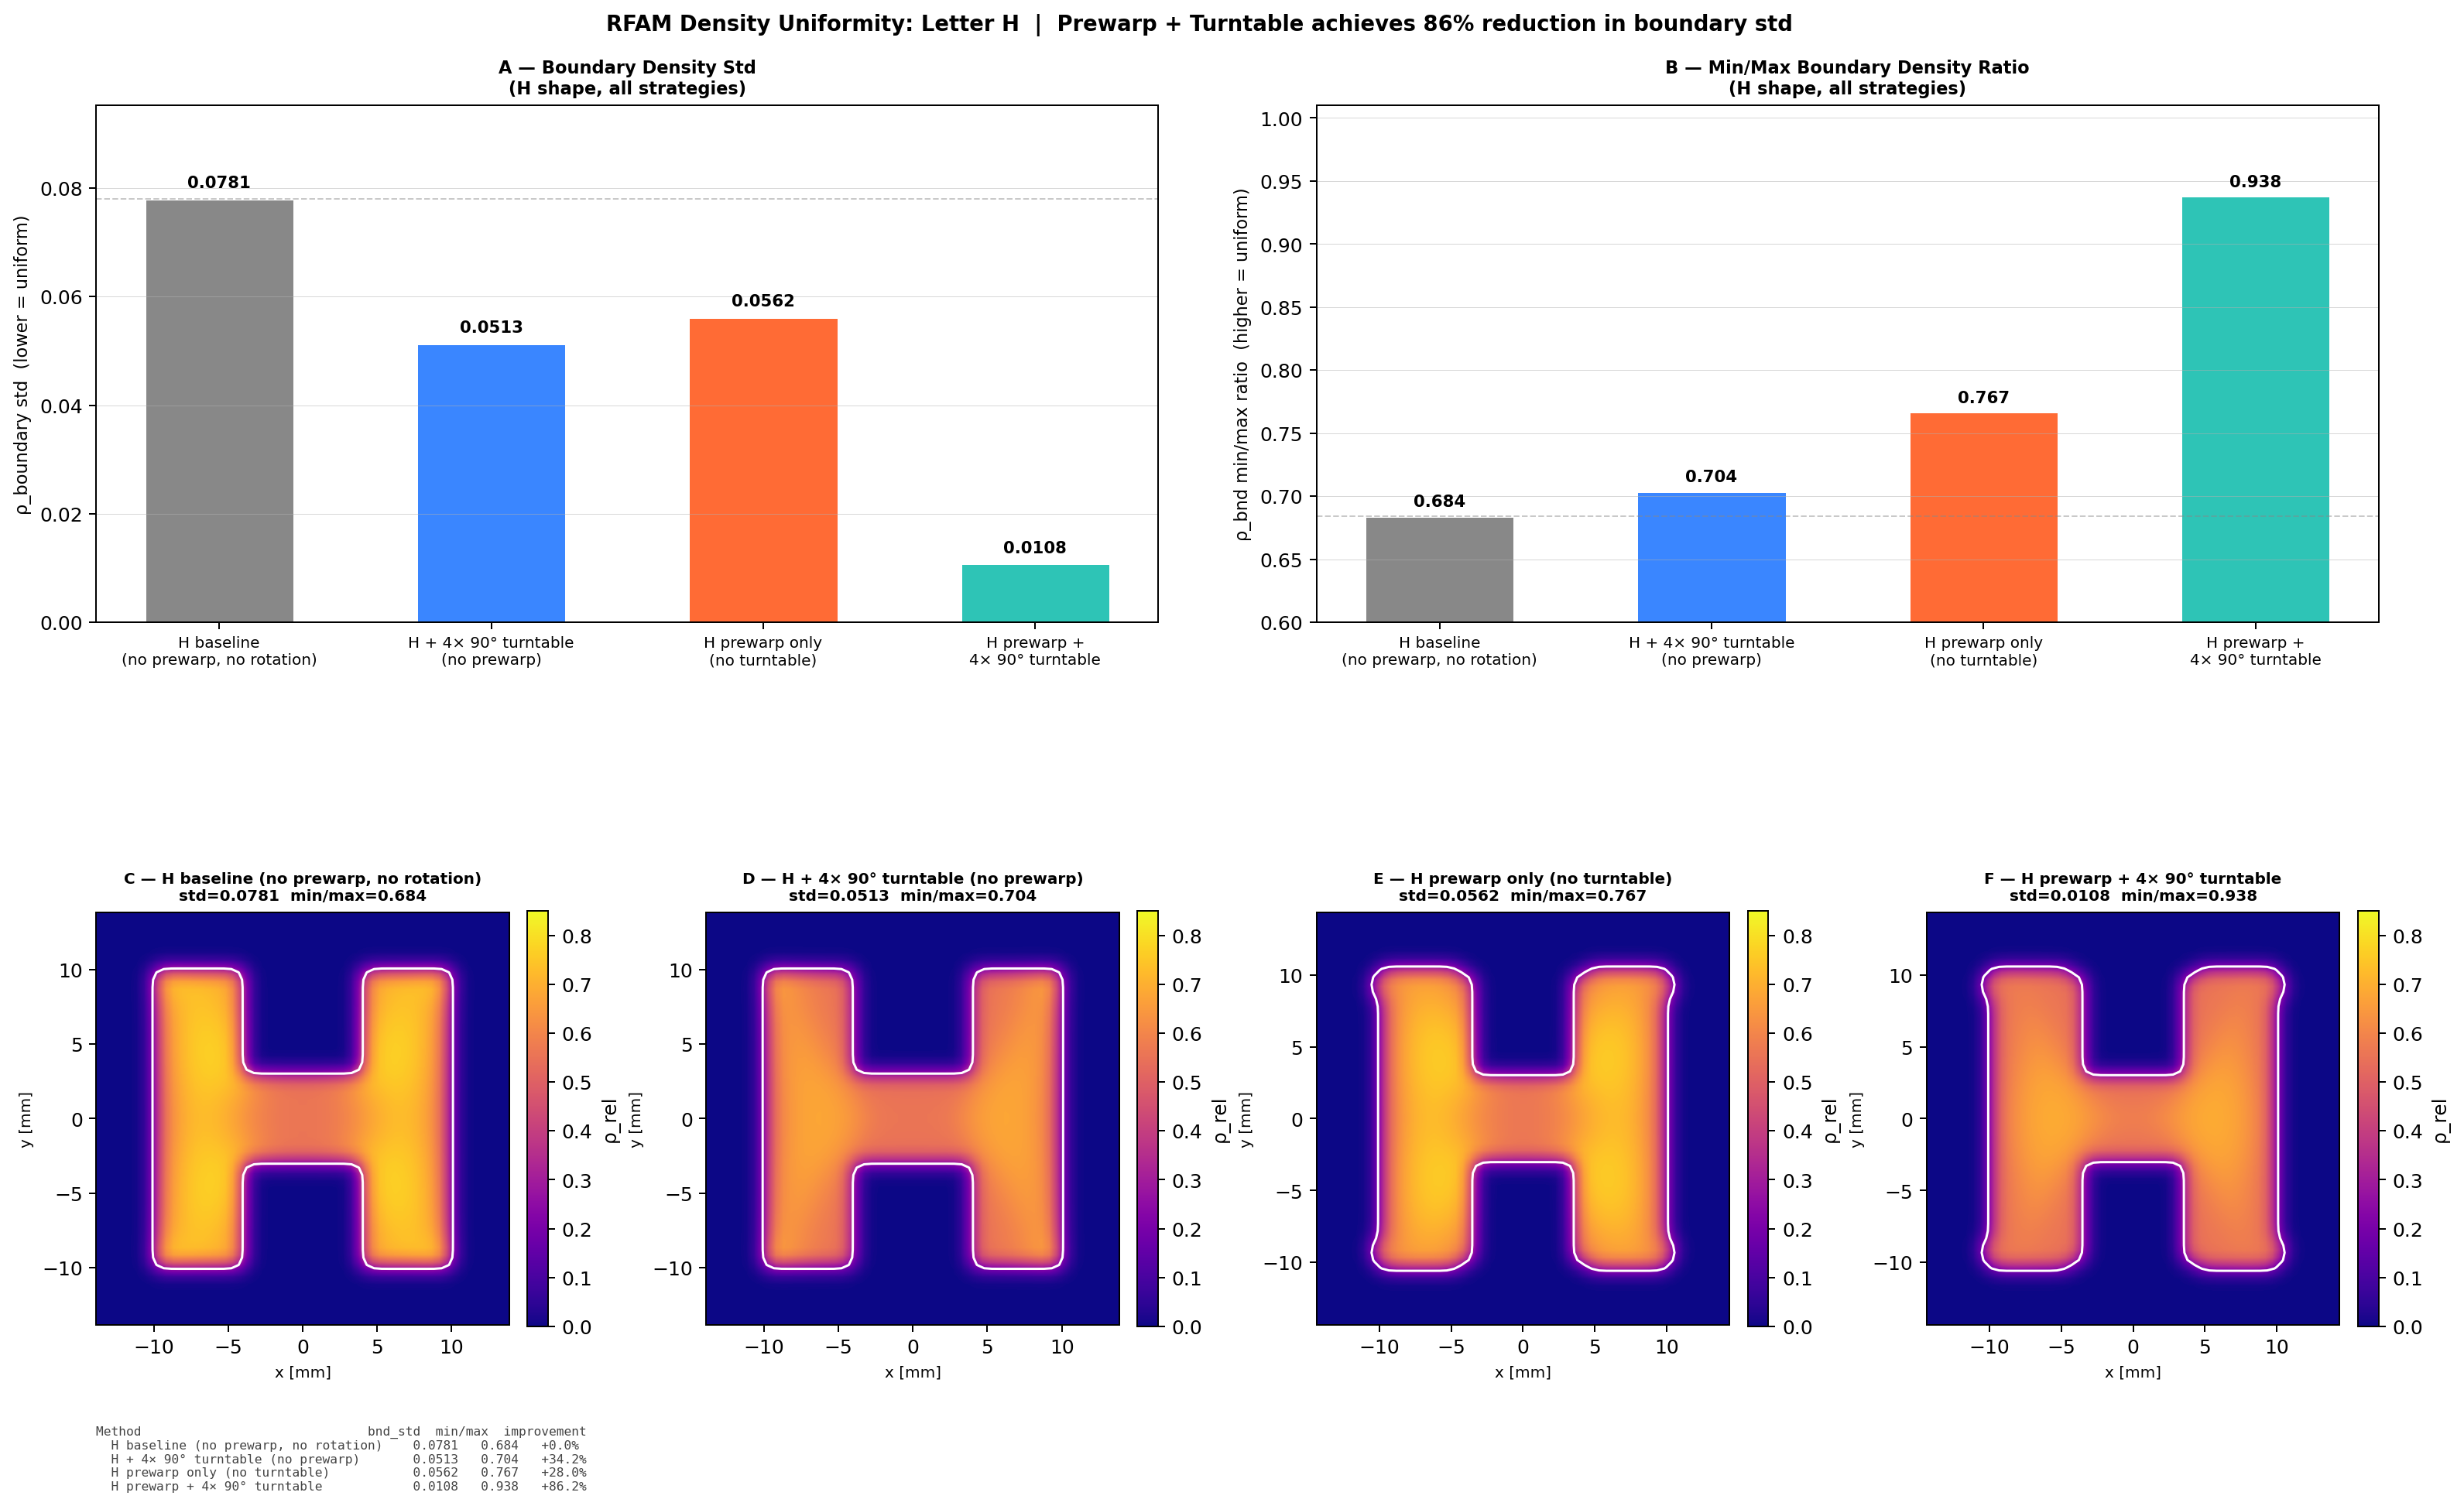
\includegraphics[width=\textwidth]{fig_H_uniformity.png}
  \caption{H-shape boundary density uniformity comparison.  Left to
           right: baseline, prewarp only, turntable only, combined
           prewarp + 4$\times$ turntable.  The combined strategy achieves
           $\bndstd = 0.011$ and $r_{\mathrm{bnd}} = 0.938$: an 86\%
           reduction in boundary density non-uniformity.  Boundary cells
           are uniformly sintered to within $\pm 1.8\%$ of the mean
           boundary density.}
  \label{fig:hshape_comparison}
\end{figure*}

\begin{figure*}[!t]
  \centering
  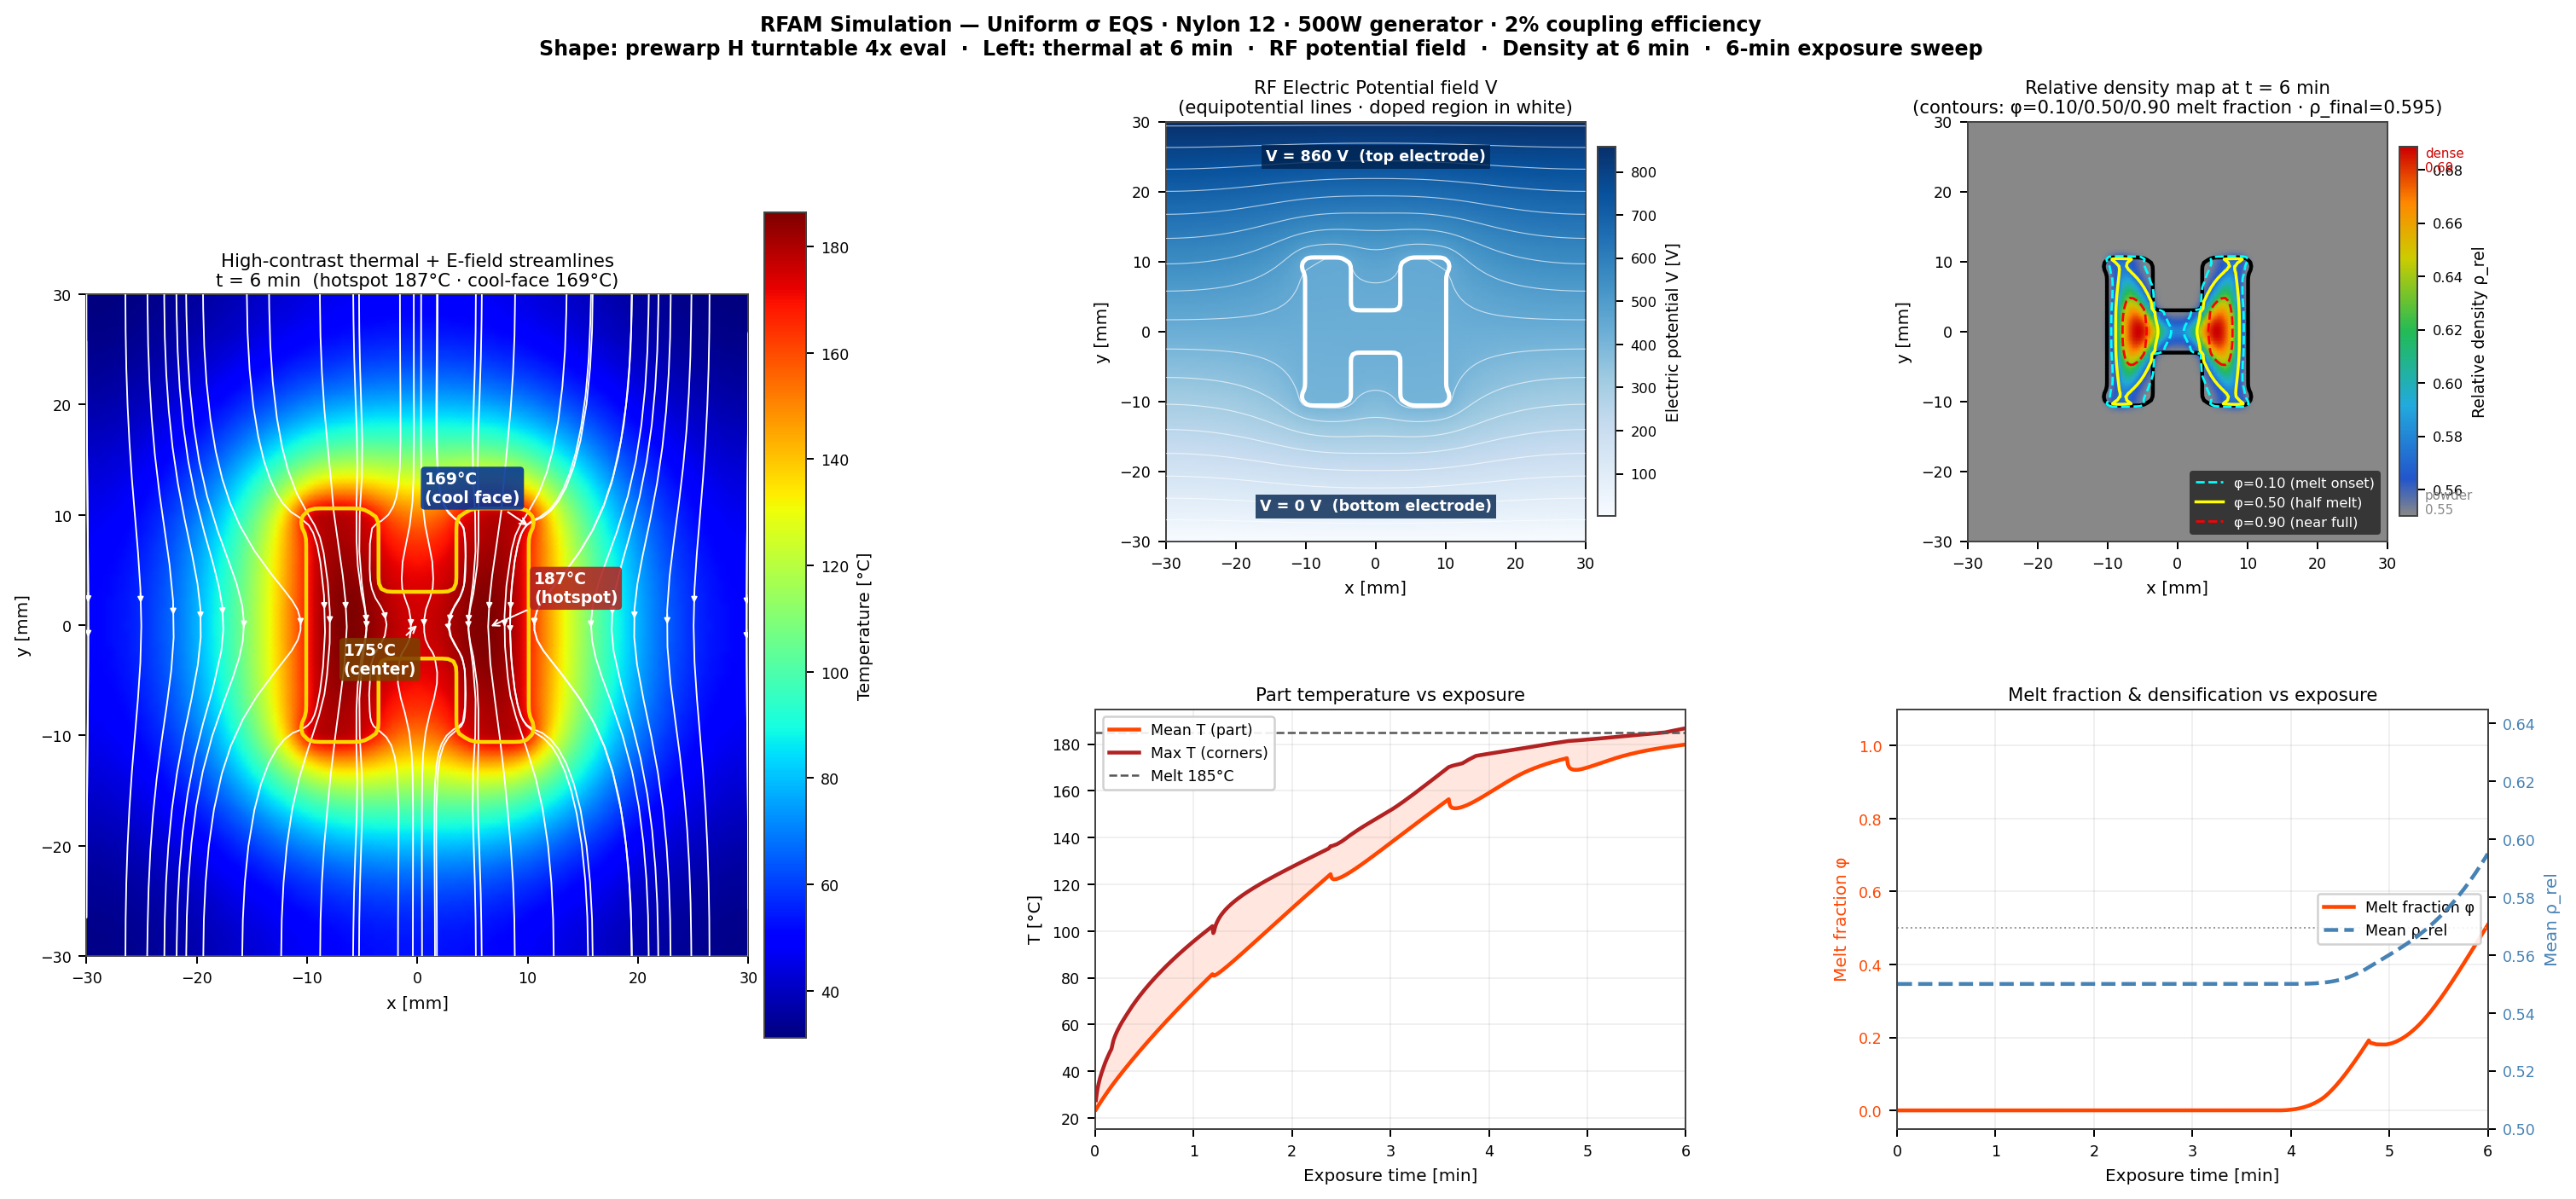
\includegraphics[width=\textwidth]{fig_H_combined_v5.png}
  \caption{Five-panel summary for the H-shape with combined prewarp +
           $4\times 90^\circ$ turntable at $t = \SI{360}{\second}$ (6 min).
           Panel layout as in \Cref{fig:canonical_full}.
           The rotational averaging is visible in the near-symmetric
           $\rhorel$ distribution (panel C): all boundary regions achieve
           $\rhorel \in [0.550, 0.586]$, a 6.5\% span, despite the
           inherent anisotropy of the RF field.
           Compare to the static baseline ($\rhorel$ span $\approx 46\%$,
           \Cref{fig:canonical_full}) to see the combined effect of
           prewarp and rotation.}
  \label{fig:hshape_combined}
\end{figure*}

\subsection{Combined H-Shape Results}

The combined prewarp + 4$\times$ turntable result for the H-shape
achieves:
\begin{itemize}
  \item $\bndstd = 0.0108$ (86.2\% reduction vs.\ baseline)
  \item $r_{\mathrm{bnd}} = 0.938$ (vs.\ 0.684 baseline)
  \item Boundary density range: $[0.550, 0.586]$ --- all boundary cells
        within 3.6\% of each other
  \item Mean temperature: $\bar{T} = \SI{179.9}{\celsius}$
\end{itemize}
\Cref{fig:hshape_comparison,fig:hshape_combined} illustrate the spatial
density distribution and the 5-panel field summary.

\subsection{Synergy Analysis: Why Combined $>$ Prewarp $+$ Turntable}

If prewarp and turntable were independent mechanisms (i.e., their
effects did not interact), the combined improvement would be
approximately the sum of their individual improvements.  For the
H-shape:
\begin{itemize}
  \item Prewarp alone: 28\% reduction in $\bndstd$
  \item Turntable alone: 34\% reduction in $\bndstd$
  \item Naive sum: 62\% expected
  \item Actual combined: 86\%
\end{itemize}
The 24-percentage-point surplus indicates a positive synergy.

The synergy arises from the following structural interaction:
\begin{enumerate}
  \item The prewarp polygon is designed for the field-anisotropic
        baseline configuration---it extends the parallel-face regions
        further outward to compensate for their lower shrinkage.  This
        creates a modified polygon with more surface area on those faces.
  \item The additional surface area at the parallel-face regions
        improves their field coupling: a face that protrudes further
        from the center encounters a slightly higher $|\vect{E}|$ and
        presents more area to field-line flux, increasing local $\Qrf$.
  \item The turntable then rotates this already-optimized polygon through
        all four $90^\circ$ orientations.  At each orientation, the
        extended face regions---which were designed for the worst-case
        (parallel) orientation---benefit equally when they rotate to
        the perpendicular orientation where they receive $11\times$
        mean coupling.
  \item The net result is that every face region alternates between
        one interval of modest coupling (parallel) and one interval of
        strong coupling (perpendicular), with the prewarp ensuring that
        the total shrinkage in each case lands exactly at the target.
\end{enumerate}
In contrast, without prewarp, the turntable rotates the unmodified
H-shape, which has equal-length faces in all orientations.  The
turntable helps, but without the geometric optimization, no face region
has a structural advantage in the parallel orientation.

\subsection{Physical Limits of the Combined Approach}

The $r_{\mathrm{bnd}} = 0.938$ achieved in the combined case implies
that boundary density ranges over only $[0.550, 0.586]$---a 6.5\% span.
The residual non-uniformity comes from two sources:

\paragraph{Discrete rotation residual.}
With 4 rotations (5 intervals of $\SI{72}{\second}$ each), one
orientation is sampled at the $0^\circ$ starting position and the
four rotated positions.  The H-shape has twofold rotational symmetry
(not fourfold), so a $90^\circ$ rotation produces a distinct field
pattern.  The resulting exposure is not perfectly uniform; a small
residual anisotropy survives.

\paragraph{Concave corner shielding.}
The H-shape's internal notch corners are shielded from the external
field regardless of rotation angle.  These cells receive heating only
by conduction from neighboring cells, which is insufficient to fully
densify them in 6 minutes.  Increasing exposure time would improve
these cells at the cost of overheating the outer corners.

%% ---------------------------------------------------------------
\clearpage
\section{L-Shape: Static Baseline, Turntable, and Orientation Optimizer}
\label{sec:lshape}
%% ---------------------------------------------------------------

\subsection{Why the L-Shape Is Diagnostically Useful}

The L-shape provides a complementary validation case to the H-shape.
Its single re-entrant corner creates a strongly shielded region
inaccessible to direct RF coupling in any orientation.  Three faces lie
approximately parallel to $\vect{E}$ and four perpendicular, producing
a large baseline coupling imbalance.  The shape has no rotational
symmetry, so every $45^\circ$ turntable step presents a geometrically
distinct field exposure, making it an ideal stress test for the
turntable averaging strategy.

\subsection{Static (Single-Orientation) Baseline}

\Cref{fig:lshape_static} shows the 8-minute single-orientation result.
The non-uniform $\rhorel$ distribution ($\overline{\rhorel} = 0.854$,
$\mathrm{UI}_\mathrm{rms} = 0.235$) reflects the parallel/perpendicular
coupling asymmetry: faces aligned with $\vect{E}$ receive substantially
less $\Qrf$ than perpendicular faces, and the re-entrant corner region
is heated only by conduction.

\begin{figure*}[!tp]
  \centering
  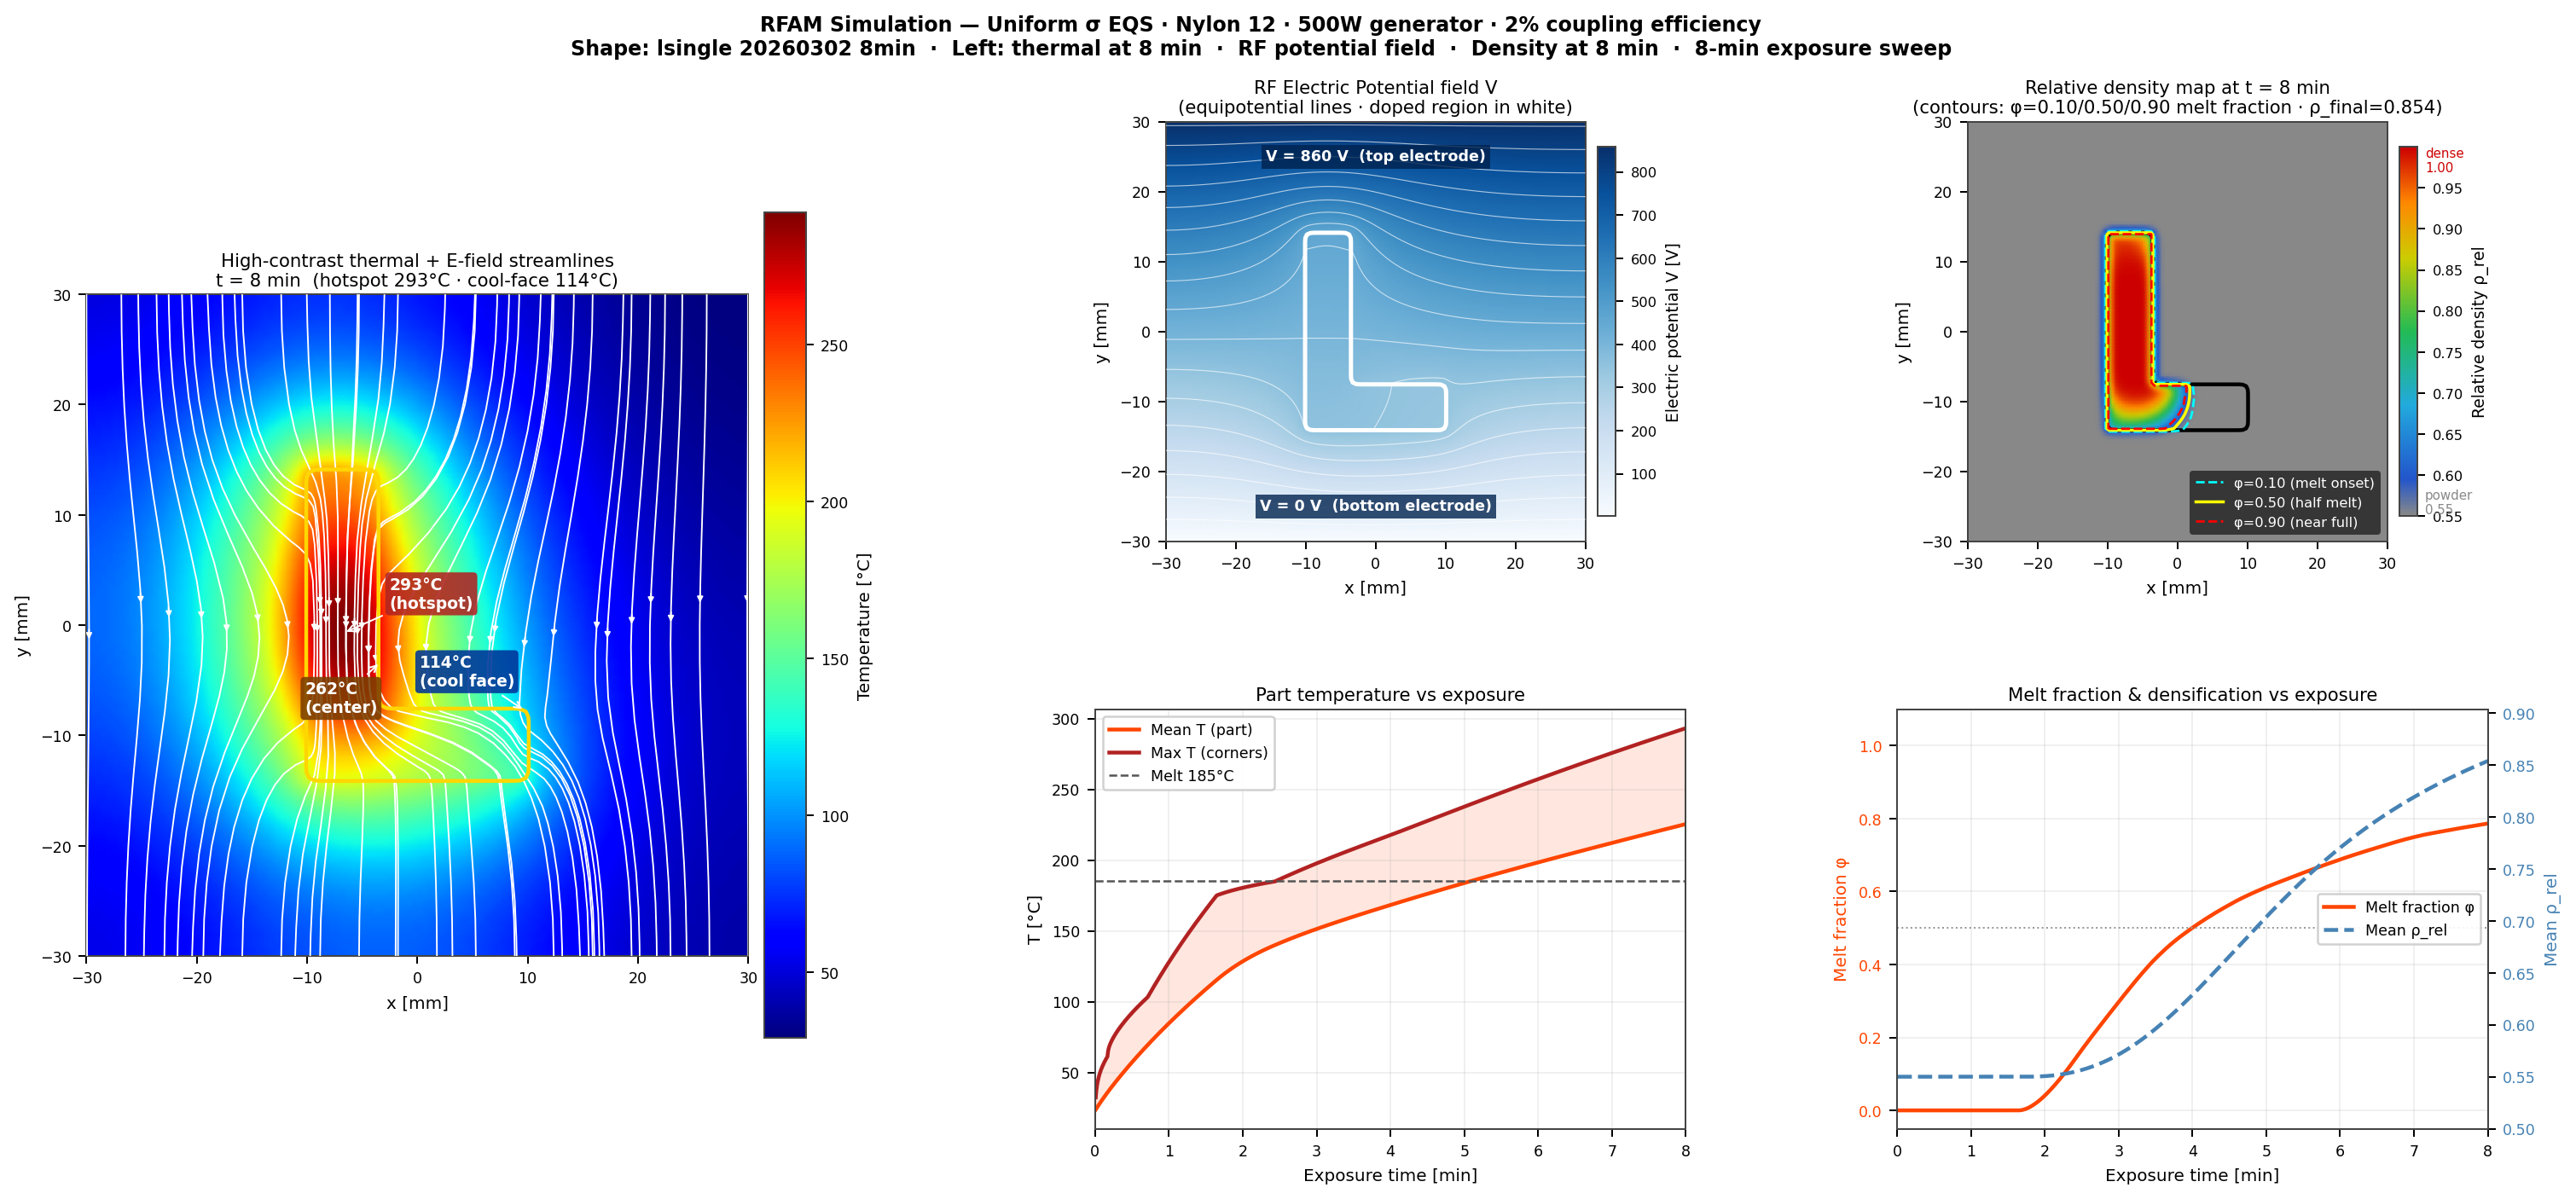
\includegraphics[width=\textwidth]{fig_lshape_static_v5.png}
  \caption{L-shape static (single orientation) result at
           $t = \SI{480}{\second}$ (8~min).  Five-panel layout as in
           \Cref{fig:canonical_full}.  Asymmetric $\rhorel$ (panel~C)
           reflects the parallel/perpendicular face coupling imbalance:
           $\overline{\rhorel} = 0.854$, $\mathrm{UI}_\mathrm{rms} = 0.235$,
           $\bar{\phimelt} = 0.786$.  The re-entrant corner (lower right in
           panel~C) receives heating by conduction only.}
  \label{fig:lshape_static}
\end{figure*}

\subsection{Turntable Result: 16$\times$ 45$^\circ$ Rotations}

Applying 16 discrete $45^\circ$ rotations over the same 8-minute exposure
(one rotation every 28~s; $720^\circ = 2$ full revolutions) substantially
homogenises the density distribution.  \Cref{fig:lshape_tt} shows the
result.  Key improvements relative to the static baseline:
\begin{itemize}
  \item $\mathrm{UI}_\mathrm{rms}$: $0.235 \to 0.126$ (46\% reduction)
  \item Mean relative density: $0.854 \to 0.899$ ($+5.2$ pp)
  \item Mean melt fraction: $0.786 \to 0.956$ ($+17$ pp)
  \item Peak temperature: $293 \to \SI{268}{\celsius}$ ($-25$~K),
        indicating more uniform heating prevents localised overheating
        at the outer corners
\end{itemize}
The dense rotation cadence averages the anisotropic $\Qrf$ pattern over
all orientations.  The re-entrant corner region retains the lowest local
density, confirming that geometric prewarp or antennae features are
needed to fully address concave shielded regions.

\begin{figure*}[!tp]
  \centering
  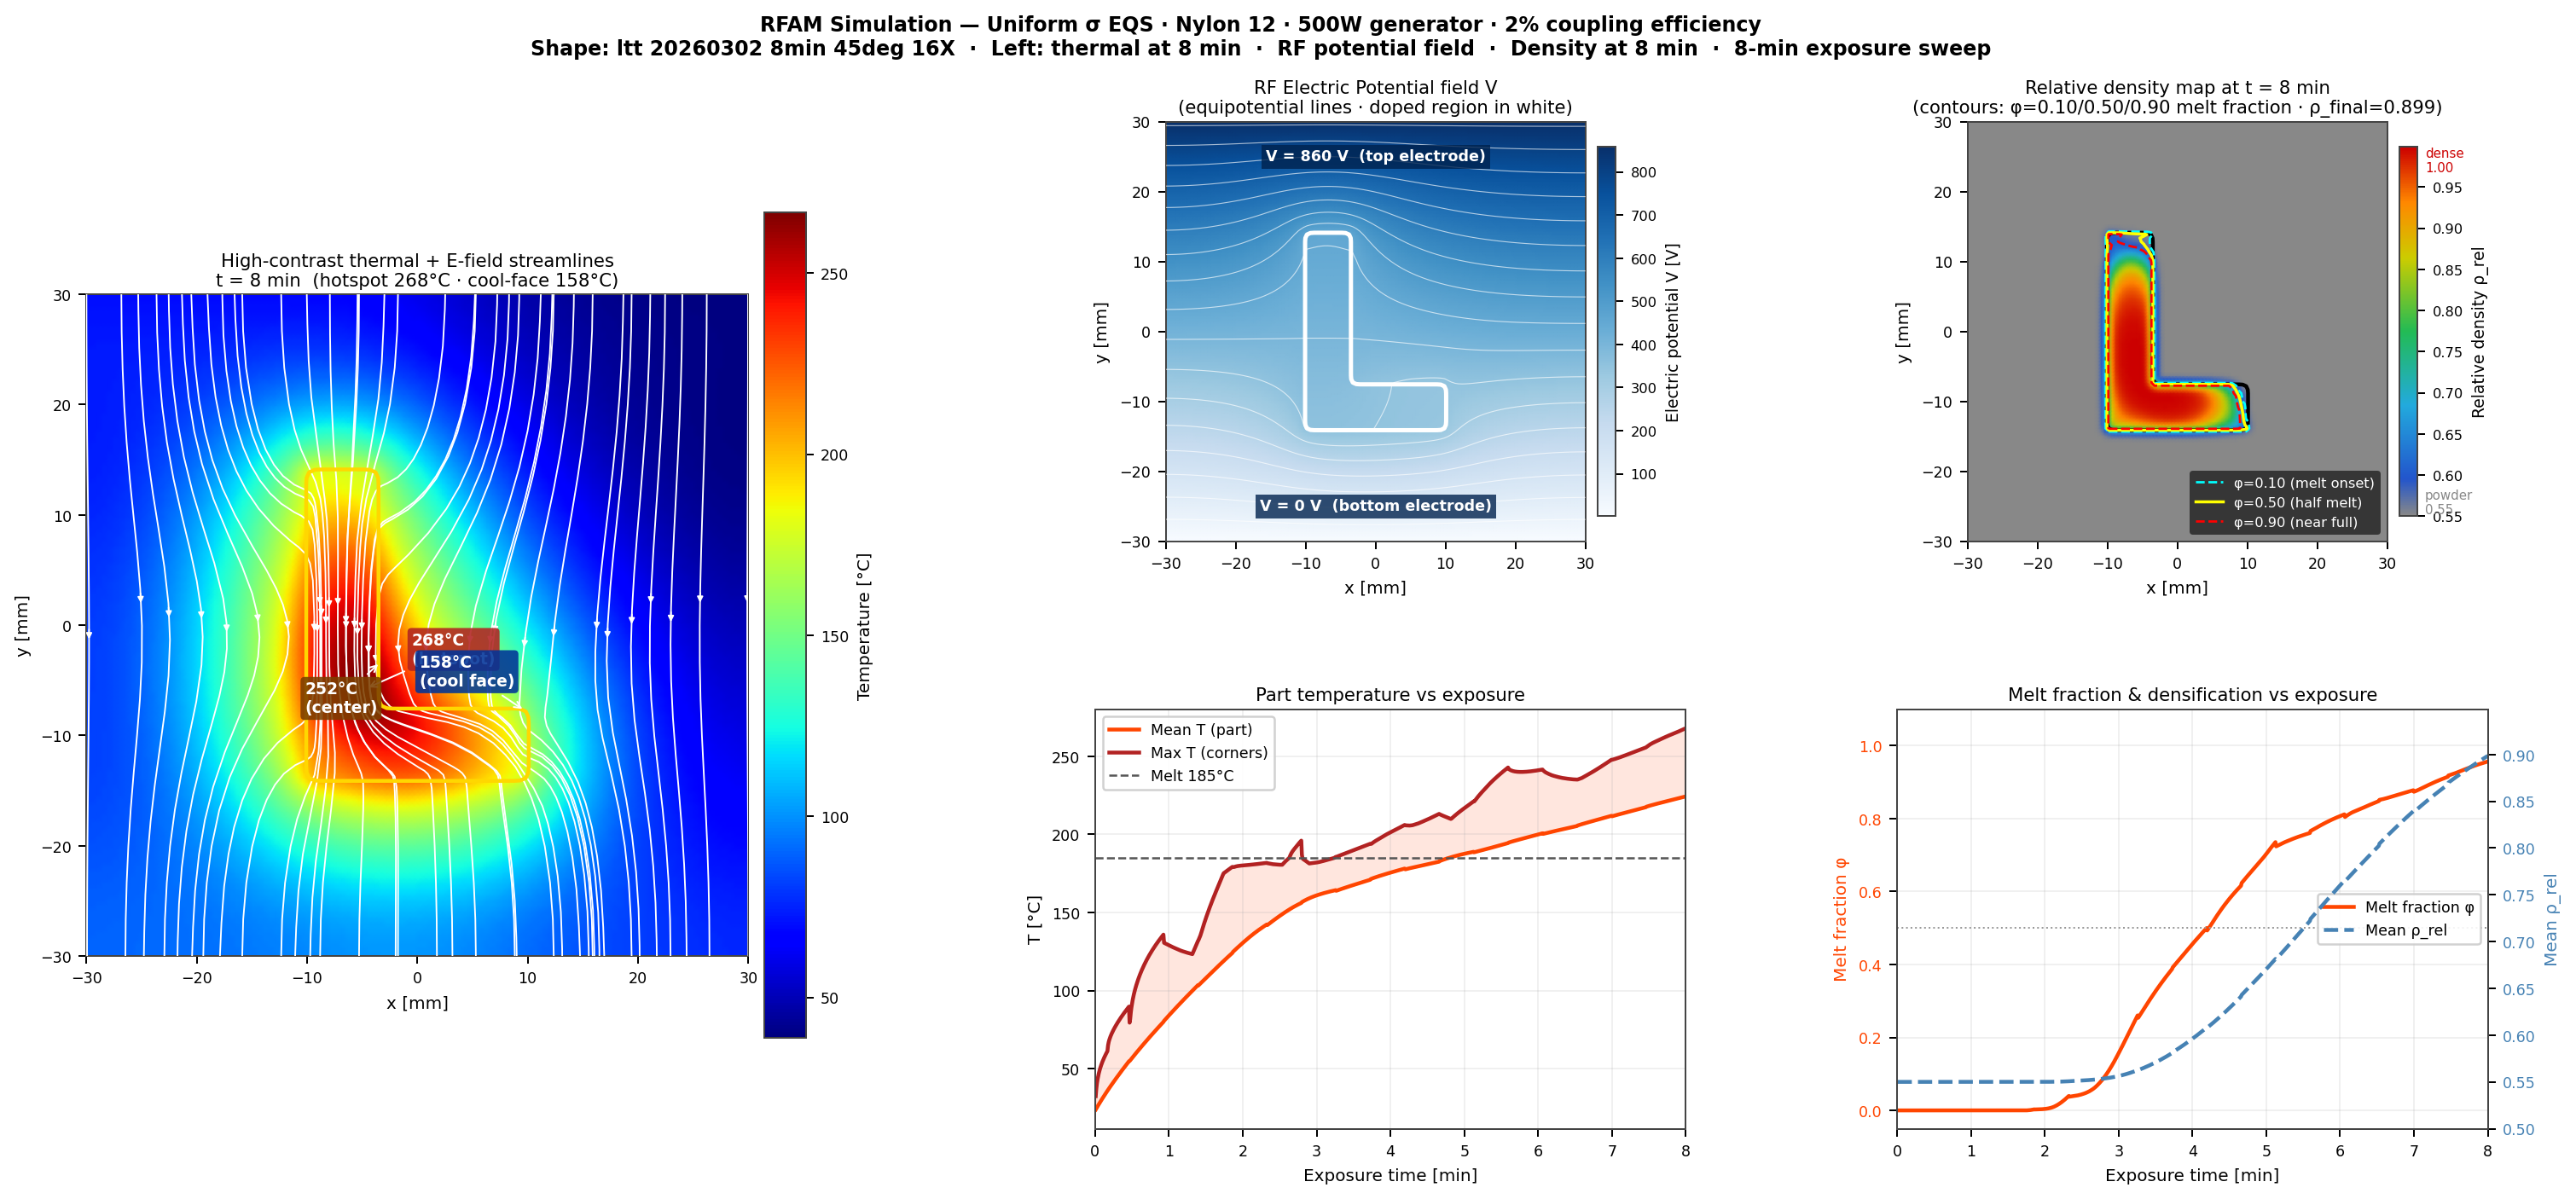
\includegraphics[width=\textwidth]{fig_lshape_tt_v5.png}
  \caption{L-shape with $16\times 45^\circ$ turntable ($720^\circ$
           total, one step every 28~s) at $t = \SI{480}{\second}$.
           Five-panel layout as in \Cref{fig:canonical_full}.
           Rotational averaging homogenises the density field (panel~C):
           $\mathrm{UI}_\mathrm{rms}$ falls from 0.235 to 0.126
           ($-46\%$), $\overline{\rhorel}$ rises to 0.899, and
           $\bar{\phimelt}$ to 0.956.  The re-entrant corner (shielded
           in all orientations) retains the lowest local density.}
  \label{fig:lshape_tt}
\end{figure*}

\subsection{Orientation Optimizer Result}

For the refreshed paper, the more practical static counterpart to the
turntable benchmark is the orientation optimizer.  Instead of rotating
the loaded chamber during exposure, the optimizer chooses a fixed part
orientation before the run, avoiding the electrode-contact problem
discussed in \cref{sec:results_turntable}.  The retained L-shape
showcase illustrates both the promise and the current limitation of
that workflow: the optimizer can identify strongly orientation-sensitive
responses, but the present objective function still tends to reward very
dense candidates even when they exceed the desired temperature ceiling.

\begin{figure*}[!tp]
  \centering
  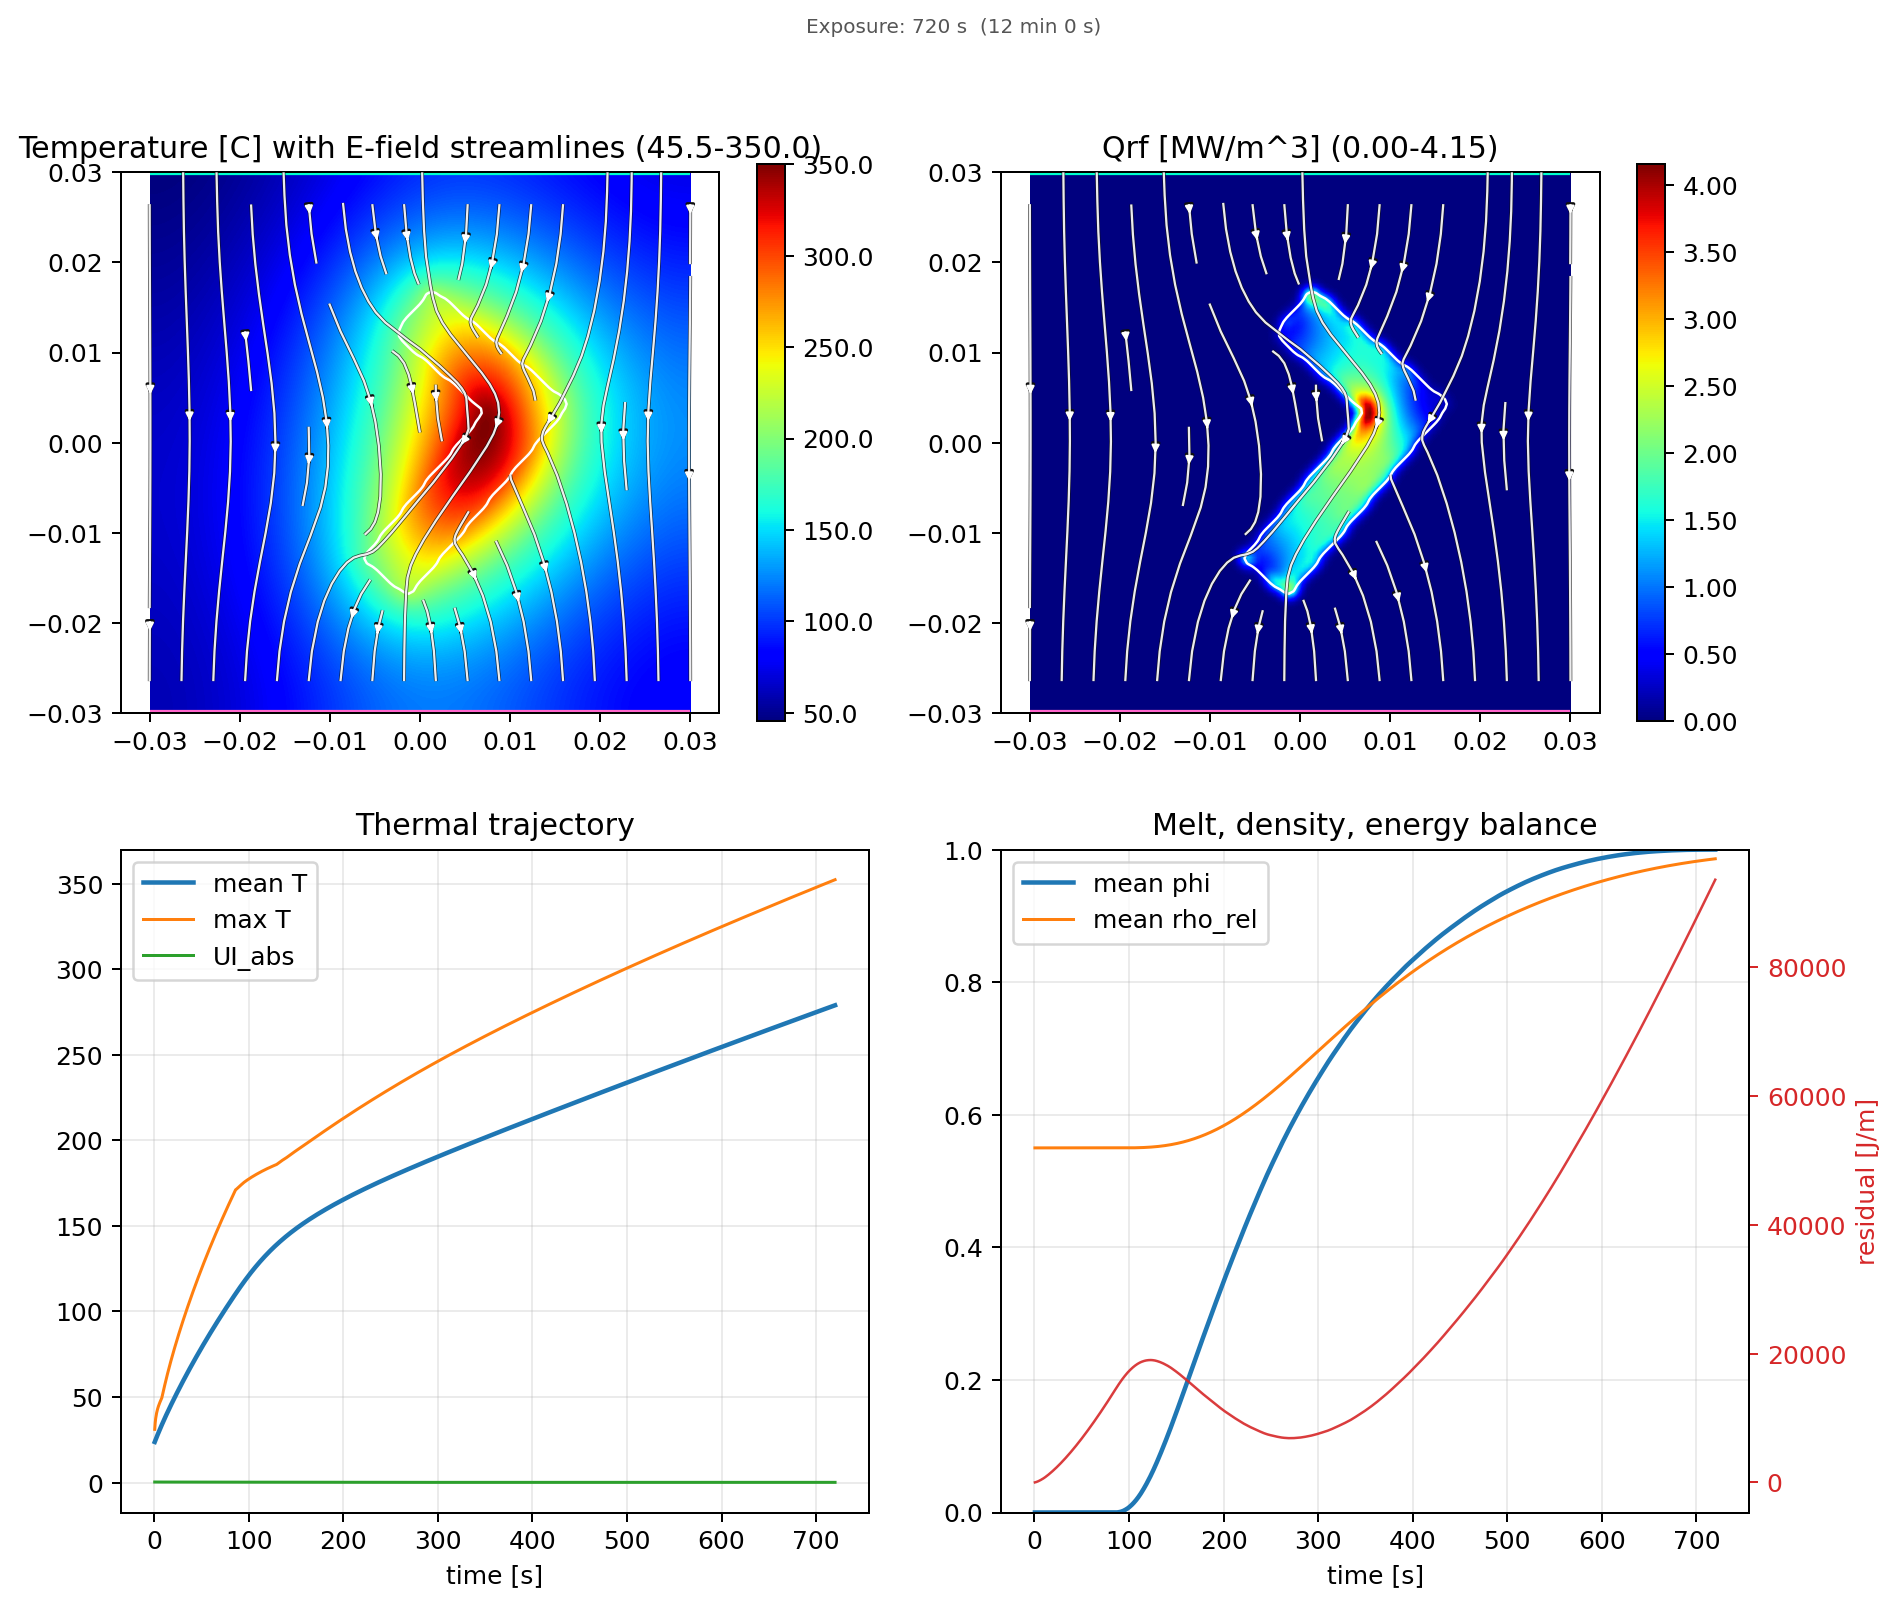
\includegraphics[width=\textwidth]{fig_orientation_lshape_refresh.png}
  \caption{L-shape orientation-optimizer showcase from the refreshed
           artifact set.  The retained report identifies a best-density
           candidate at a rotated orientation, but it also makes clear
           that the current optimizer objective still allows large
           temperature-ceiling violations.  This is therefore presented
           as the practical next development path, not as a fully solved
           workflow.}
  \label{fig:lshape_opt}
\end{figure*}

\begin{table}[tb]
\centering
\caption{L-shape orientation-optimizer showcase used in the refreshed manuscript. This section is framed as the more practical static alternative to a physical turntable because it avoids breaking electrode/media contact during the run.}
\label{tab:orientation_refresh}
\small
\begin{tabular}{lr}
\toprule
Metric & Value \\
\midrule
Best angle [deg] & 140.0 \\
Exposure [s] & 720 \\
Mean $\rho_{rel}$ & 0.986 \\
Max temperature [C] & 352.3 \\
Temperature ceiling violation [C] & 102.3 \\
Energy residual [\%] & 26.00 \\
\bottomrule
\end{tabular}
\end{table}

%% ---------------------------------------------------------------
\FloatBarrier
\section{Discussion}
\label{sec:discussion}
%% ---------------------------------------------------------------

\subsection{Model Validation and Calibration}

The refreshed forward model now carries more calibrated structure than
the older draft emphasized.  In addition to the electrical loading
parameters $\sigma = \SI{0.04}{\siemens\per\meter}$ and $\eta = 0.020$,
the main March~2026 workflow also depends on the DSC melt profile and
the viscous-capillary PA12 densification parameters used by the default
model family.  The main validation point remains that the model
reproduces the expected corner/face/center heating hierarchy, but the
paper now supplements that interpretation with explicit error columns
rather than implying that a visually plausible field pattern is by
itself sufficient.

The key simplification relative to COMSOL is the uniform $\sigma$
approximation.  The COMSOL reference model (Tuned\_Sigma.mph,
from~\cite{allison2022computational,allisonDissertation}) uses a
spatially varying conductivity with the characteristic \emph{shell}
pattern (high at outer faces/edges, low at the center), resulting in
an average $\sigma \ll \SI{0.04}{\siemens\per\meter}$.  The Python
model compensates for this by setting $\eta = 0.020$, which reduces
the effective absorbed power to match the COMSOL result.  The spatial
pattern of $\Qrf$ in both models shows the same corner-to-face-to-center
hierarchy (\cref{fig:canonical_fields,fig:canonical_full}), confirming
that the dominant spatial structure is driven by geometry (boundary
conditions) rather than by the $\sigma$ distribution.

\subsection{Comparison to Optical ILT}

The EPE-based prewarp algorithm is directly analogous to standard ILT
methods~\cite{zhang2023fast,zhu2024l2o,poonawala2007mask}, with three key differences:

\paragraph{Forward model complexity.}
Optical ILT uses an analytical or semi-analytical forward model for the
aerial image (Hopkins or Abbe formulation); this enables analytic
gradient computation and fast optimization.  The RFAM forward model
requires a full PDE solve ($\approx$\SI{30}{\second} per iteration on a
laptop).  Consequently, the RFAM prewarp can afford only 2--3 iterations,
whereas optical ILT may run hundreds.

\paragraph{Binary vs.\ continuous mask.}
Optical masks are binary (opaque/transparent); the prewarp polygon is
a continuous boundary.  The RFAM analog of the mask is the input
polygon, which is free to take any shape---there is no tone
constraint.  This makes the RFAM problem in some ways easier
(continuous design space) and in some ways harder (no natural
binarization to prevent over-complicated geometries).

\paragraph{Shrinkage nonlinearity.}
The optical aerial image is related to the mask by a linear
convolution; the sintered boundary is related to the input polygon by
a nonlinear, history-dependent PDE system.  The Arrhenius densification
kinetics and phase-change latent heat introduce strong nonlinearities
that prevent the use of gradient-based optical ILT algorithms without
significant modification.

\subsection{Practical Implementation Considerations}

\paragraph{Rotation actuator.}
The key challenge is not merely rotating a stage; it is rotating the
loaded powder/part medium while preserving the intended contact
condition at the electrode-facing boundaries.  If the motion introduces
an effective air gap, the RFAM chamber behaves more like a different
impedance network than like the intended load.  This is why the
refreshed paper treats the turntable primarily as a benchmark and
positions the static orientation optimizer as the more practical
near-term deployment path.

\paragraph{Prewarp pipeline.}
In a production RFAM workflow, the prewarp algorithm would run
offline prior to printing.  The 2--3 forward model evaluations required
for convergence ($\approx\SI{1}{\minute}$ each on the target hardware)
represent a modest pre-computation cost.  The converged prewarp polygon
replaces the original part outline in the binder-jetting layer mask,
requiring no changes to the RF exposure hardware.

\paragraph{3D extension.}
The current model is 2D (cross-section in the XZ plane).  Real parts
have a finite out-of-plane dimension and 3D E-field structure.  The
2D model is exact for infinitely long parts in the Y-direction and is
an approximation for parts with finite aspect ratios.  The 3D
generalization would require a 3D EQS solve (much higher computational
cost) and a 3D prewarp algorithm (vertex update in 3D with surface
normal computation on a mesh).  The turntable strategy extends directly
to 3D by rotating about the Z-axis (perpendicular to the electrode
faces).

%% ---------------------------------------------------------------
\FloatBarrier
\section{Conclusions}
\label{sec:conclusions}
%% ---------------------------------------------------------------

This paper has refreshed the RFAM compensation study around the current
HEATR physics stack while preserving the original structure of the
manuscript.  The following conclusions are supported by the updated
figures, tables, and discussion:

\begin{enumerate}

\item \textbf{Current HEATR physics description.}  The RFAM solver used
      for the refreshed mainline results is now described correctly as
      a complex-coefficient EQS solve with generator-power scaling, a
      DSC-calibrated apparent-heat-capacity PA12 phase model,
      viscous-capillary densification, and explicit validation/error
      diagnostics.

\item \textbf{EPE prewarp convergence.}  The EPE-gradient-descent
      prewarp algorithm converges in 2--3 iterations to geometric RMSE
      below \SI{0.25}{\milli\meter} for simple shapes (circle, square)
      and below \SI{0.30}{\milli\meter} for complex shapes (H), starting
      from geometric RMSE of 0.37--\SI{0.68}{\milli\meter}.  This
      represents a 59--68\% reduction in geometric RMSE.

\item \textbf{$\Leff$ calibration.}  The optimal effective shrinkage
      length is $\SI{5}{\milli\meter}$ for the circle and
      $\SI{7}{\milli\meter}$ for the square and H-shape.  Physically,
      $\Leff$ relates to the characteristic sintering diffusion length
      at 6 minutes exposure; the higher value for shapes with sharp
      corners reflects the three-dimensional material redistribution
      at vertices that is not captured by the 2D model.

\item \textbf{Shape library refresh.}  The 17-geometry single-exposure
      screen remains a useful first-order map of geometry sensitivity,
      but the refreshed paper now reports those results together with
      the solver-error context rather than as standalone performance
      numbers.

\item \textbf{Antennae energy concentrators remain exploratory.}  The
      limited square-study calibration set currently available in the
      repository is not yet compelling enough to support a strong claim
      of benefit.  The paper now treats this idea as a future DOE topic
      rather than as a mature correction strategy.

\item \textbf{Turntable rotation is still useful, but mainly as a
      benchmark.}  The refreshed multi-geometry comparison confirms that
      discrete rotation can reduce boundary-density anisotropy, but the
      hardware constraint of maintaining electrode/media contact means
      that a physical turntable is not necessarily the preferred
      deployment path.

\item \textbf{Orientation optimization is the practical next step.}
      The retained L-shape showcase demonstrates that static orientation
      selection can capture much of the same geometric insight as a
      turntable benchmark without requiring in-process chamber
      rotation.  The remaining task is to tighten the optimizer
      objective so that temperature-ceiling violations are penalized
      more strongly.

\end{enumerate}

Future work will address: (a) 3D extension of the EQS and prewarp
models; (b) experimental validation against sintered Nylon~12 parts;
(c) a full refresh of the prewarp workflow on the DSC-calibrated model
family; (d) a structured DOE for antennae energy concentrators; and
(e) improved orientation / turntable objective functions with tighter
solver-quality gating.

%% ---------------------------------------------------------------
\section*{Acknowledgments}
%% ---------------------------------------------------------------

The author thanks Prof.\ Christopher Seepersad for guidance on RFAM
process physics and C.B.\ Allison for the COMSOL reference model.
This work was supported by the Georgia Institute of Technology School
of Mechanical Engineering.

%% ---------------------------------------------------------------
%% References  (BibTeX — compile with pdflatex → bibtex → pdflatex × 2)
%% ---------------------------------------------------------------
\bibliographystyle{elsarticle-num}
\bibliography{references}

\end{document}
